%!TEX root=tese.tex
\chapter{Fundamentos Práticos} % (fold)
\label{cha:pra}
Neste capítulo são abordados os principais fundamentos, de carácter prático, no âmbito do presente trabalho. Devido à elevada diversidade de materiais e métodos utilizados na realização dos trabalhos experimentais, descritos nos capítulos~\ref{chap:art1}--\ref{chap:art4}, não seria viável fazer a sua exposição no presente capítulo. Assim, os detalhes experimentais específicos de cada trabalho são expostos no seu capítulo correspondente, ficando remetidos para o presente capítulo os detalhes experimentais que possuem uma aplicação mais transversal no âmbito do presente trabalho. Na seguinte secção é descrito o principal equipamento de filtração utilizado, nomeadamente a célula de filtração Amicon 8010.   

\section{Célula de filtração Amicon 8010} % (fold)
\label{sec:amicon}\index{Amicon 8010}%
Nesta secção descreve-se a principal célula de filtração usada, a célula de filtração Amicon 8010 (\emph{Millipore}). Esta célula, ilustrada na figura~\ref{fig:amicon}, tem uma geometria ``dead-end'', isto é, o fluxo de filtração apresenta uma direção perpendicular à superfície da membrana, membrana esta que é assente num suporte horizontal que contém um orifício por onde é recolhido o permeado. Para melhorar o coeficiente de transferência de massa, a célula dispõe de um agitador magnético que atua perto da superfície da membrana.\index{dead@``dead-end''}\index{agitador magnético} 

A célula pode ser operada de duas formas distintas (figura~\ref{fig:amicon}). Pode ser conectada a uma fonte de pressão (usualmente azoto ou ar comprimido), pressão esta que força o líquido a permear pela membrana. O fluxo de filtração não é facilmente controlável por este método, apenas o valor do diferencial de pressão através da membrana pode ser estabelecido de forma precisa. Este facto dificulta a tentativa de modelar matematicamente a filtração dado que o fluxo de filtração é um parâmetro crucial na formulação dos modelos teóricos apresentados no capítulo~\ref{chap:teov3}. Por outro lado, este método apresenta-se como o mais eficiente para efetuar alguns tipos de procedimentos, como a lavagem de membranas e a determinação das suas permeabilidades hidráulicas.\index{permeabilidade hidráulica}\index{fluxo!filtração}\index{pressão}
\begin{figure}
\centering
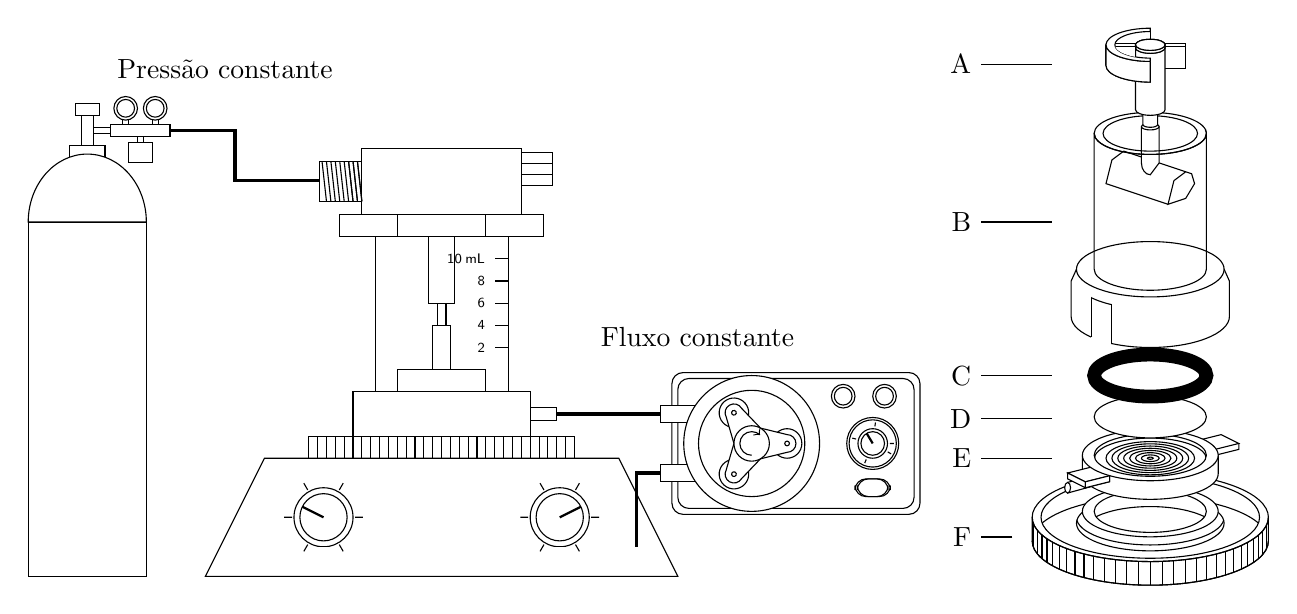
\begin{tikzpicture}[decoration={ticks,amplitude = 0.025cm}]

%%ESQUEMA DE MONTAGEM AMICON 8010
%% BASE
\begin{scope}[scale=0.75,xshift=17cm]
\draw (2cm,1cm) ellipse (2cm and 0.75cm);
\begin{scope}
\clip[draw] (2cm,1cm) ellipse (1.85cm and 0.69375cm);
\draw (0cm,0.6cm) arc (180:0:2cm and 0.75cm);
\end{scope}
\draw (0cm,0.6cm) arc (-180:0:2cm and 0.75cm);
\draw (4cm,1cm) -- (4cm,0.6cm);
\draw (0cm,1cm) -- (0cm,0.6cm);
\begin{scope}
\clip[draw] (4cm,0.6cm) arc (0:-180:2cm and 0.75cm) -- (0cm,1cm) arc (-180:0:2cm and 0.75cm)--cycle;
\foreach \x in {%
2.00000,%
2.20000,%
2.39850,%
2.59254,%
2.77938,%
2.95660,%
3.12228,%
3.27505,%
3.41409,%
3.53910,%
3.65027,%
3.74814,%
3.83354,%
3.90747,%
3.97103}%
\draw[thin] (\x,1cm) -- (\x,-0.5cm);
\foreach \x in {%
1.80000,%
1.60150,%
1.40746,%
1.22062,%
1.04340,%
0.87772,%
0.72495,%
0.58591,%
0.46090,%
0.34973,%
0.25186,%
0.16646,%
0.09253,%
0.02897}%
\draw[thin] (\x,1cm) -- (\x,-0.5cm);
\end{scope}
\draw (2cm,0.9cm) ellipse (1.25cm and 0.46875cm);
\filldraw[fill=white,draw=black] (2cm,1.1cm) ellipse (1.15cm and 0.43125cm); 
\begin{scope}
\clip[draw] (2cm,1.1cm) ellipse (0.95cm and 0.356cm); 
\draw (2cm,0.75cm) ellipse (1.15cm and 0.43125cm); 
\end{scope}
\begin{scope}
\clip (2cm,0.9cm) ellipse (1.25cm and 0.46875cm);
\draw (0.75cm,1cm) arc (-180:0:1.25cm and 0.46875cm);
\end{scope}
% fim base

% Suporte
\begin{scope}[yshift=-0.95cm]
\fill[white] (2cm,2.685cm) ellipse (1.15cm and 0.43125cm);
\filldraw[fill=white,draw=black] (0.6,2.54)--(1,2.65)--(1,2.47)--(0.6,2.36)--cycle;
\filldraw[fill=white,draw=black] (0.6,2.45) ellipse (0.05 and 0.09);
\draw (0.85cm,3cm) -- (0.85cm,2.685cm) arc (-180:0:1.15cm and 0.43125cm) -- (3.15cm,3cm);
\filldraw[fill=white,draw=black] (0.9cm,2.55cm)--(3.5cm,3.20cm)--(3.2cm,3.35cm)--(0.6,2.7)--cycle;
\filldraw[fill=white,draw=black] (0.6,2.7) -- (0.6,2.6)--(0.9,2.45)--(0.9,2.55)--cycle;
\draw (3.5,3.2)--(3.5,3.1)--(2,2.725);
\draw (0.9,2.45)--(1.3125,2.553125)--(1.3125,2.653125);
\filldraw[fill=white,draw=black](2cm,3cm) ellipse (1.15cm and 0.43125cm); 
\begin{scope}
\clip[draw] (2cm,3cm) ellipse (0.95cm and 0.356cm);
\draw (2cm,2.935cm) ellipse (0.95cm and 0.356cm);
\end{scope}
\draw(2cm,2.95cm) ellipse (0.75cm and 0.28125cm); 
\draw (2cm,2.95cm) ellipse (0.6500cm and 0.2437cm);
\draw (2cm,2.95cm) ellipse (0.5500cm and 0.2062cm);
\draw (2cm,2.95cm) ellipse (0.4500cm and 0.1687cm);
\draw (2cm,2.95cm) ellipse (0.3500cm and 0.1312cm);
\draw (2cm,2.95cm) ellipse (0.2500cm and 0.0937cm);
\draw (2cm,2.95cm) ellipse (0.1500cm and 0.0562cm);
\draw (2cm,2.95cm) ellipse (0.0500cm and 0.0187cm);
\filldraw[fill=white,draw=black] (0.9,2.55)--(0.9,2.45)--(1.3125,2.553125)--(1.3125,2.653125)--cycle;
\end{scope}
% end suporte

% Membrana
\begin{scope}[yshift=-1.8cm]
\filldraw[fill=white,draw=black] (2cm,4.5cm) ellipse (0.95cm and 0.356cm);
\end{scope}
% fim membrana

% O-ring
\begin{scope}[yshift=-2.6cm]
\draw[line width=5pt] (2cm,6cm) ellipse (0.95cm and 0.356cm);
\end{scope}
% fim o-ring

% body
\begin{scope}[yshift=-1.5cm]
\draw (2,6.7) ellipse (1.25cm and 0.46875cm);
\draw (0.75,6.7)--(0.66,6.5);
\draw (0.66,6.5)--(0.66,5.9) arc (-180:0:1.34 and 0.525)--(3.34,6.5);
\draw (3.25,6.7)--(3.34,6.5);
\draw (2,9) ellipse (0.95cm and 0.356cm);
\draw (2,9) ellipse (0.8cm and 0.3cm);
\draw (1.05,9) -- (1.05,6.7) arc (-180:0:0.95cm and 0.356cm)--(2.95,9) arc (0:-180:0.95cm and 0.356cm)--cycle;
\begin{scope}
\clip (1,6.1)rectangle(1.35,6.25);
\draw (2,6.5) ellipse (1.25cm and 0.46875cm);
\end{scope}
\fill[white] (1,5.43) rectangle (1.35,5.56);
\draw (1,5.550536444)--(1,6.21875) (1.35,6.099609566)--(1.35,5.440901801);
\end{scope}
% end body

% magnetic stirrer
\begin{scope}[yshift=-3cm]
\draw (2,10.615) ellipse (0.15cm and 0.05625cm);
\draw (1.85,10.615) -- (1.85,10) arc (-180:-90:0.15cm and 0.2cm)--(2.15,10)--(2.15,10.615);
\draw (2.15,10)--(2.6,9.85)--(2.4,9.7)--(2.3,9.3)--(2.6,9.4)--(2.75,9.65)--(2.7,9.8167)--cycle;
\draw (2.3,9.3) -- (1.25,9.65)--(1.35,10.05)--(1.55,10.20)--(1.85,10.1);
\filldraw[fill=white,draw=black] (1.875,11)--(1.875,10.65) arc (-180:0:0.125cm and 0.046875cm)--(2.125,11)--cycle;
\filldraw[fill=white,draw=black] (1.75,12)--(1.75,10.9) arc (-180:0:0.25cm and 0.09375cm) -- (2.25,12)--cycle;
\filldraw[fill=white,draw=black] (2,11.95) ellipse (0.25cm and 0.09375cm);
\filldraw[fill=white,draw=black] (2,12) ellipse (0.25cm and 0.09375cm);
\draw (2,12.281245)--(2,11.931245);
\draw (2,11.775)--(2,11.425);
\draw (2,11.931245) arc (90:270:0.75cm and 0.281245cm)--(2,11.718755);
\draw (1.25,11.65)--(1.25,12);
\filldraw[fill=white,draw=black] (2,11.95) ellipse (0.25cm and 0.09375cm);
\filldraw[fill=white,draw=black] (2,12) ellipse (0.25cm and 0.09375cm);
\filldraw[fill=white,draw=black] (1.25,12)--(1.25,11.65) arc (180:270:0.75cm and 0.281245cm) -- (2,11.718755)%
arc (-90:-180:0.75cm and 0.281245cm) --cycle;
\filldraw[fill=white,draw=black] (2,11.718755)--(2,11.775) arc (270:90:0.6cm and 0.225cm) -- (2,12.281245)%
arc (90:270:0.75cm and 0.281245cm) -- cycle;
\begin{scope}
\clip (2,12) ellipse (0.6cm and 0.225cm);
\draw (1,12.025)--(2,12.025);
\filldraw[fill=white,draw=black] (1,11.975)--(1.75,11.975)--(1.75,11.5)--(1,11.5)--cycle;
\end{scope}
\draw (2,12.025)--(2.6,12.025)--(2.6,11.975)--(2,11.975);
\draw (2.6,11.975)--(2.6,11.6)--(2.25,11.6);
\filldraw[fill=white,draw=black] (2,12) ellipse (0.25cm and 0.09375cm);
\end{scope}
% end magnetic stirrer
\end{scope}
%% FIM ESQUEMA AMICON 8010


%% ESQUEMA DE UTILIZAÇÃO AMICON 8010
\begin{scope}[scale=0.75]
\begin{scope}[xshift=-3cm]
% amicon 8010
\begin{scope}[xshift=10cm,yshift=2cm,xscale=0.75,yscale=0.75]
\foreach \x in {-2.8,-2.6,...,2.8} \draw (\x,0) -- (\x,0.5);
\draw (-1,5) -- (-1,5.5);
\draw (1,5) -- (1,5.5);
% Graduação do corpo
\draw (1.5,4.5) -- (1.2,4.5) ;
\node [left,font=\tiny] at (1.2,4.5) {$\mathsf{10\,mL}$};
\draw (1.5,4) -- (1.2,4) ;
\node [left,font=\tiny] at (1.2,4)  {$\mathsf{8}$ };
\draw [font=\tiny] (1.5,3.5) -- (1.2,3.5) ;
\node [left,font=\tiny] at (1.2,3.5)  {$\mathsf{6}$ };
\draw [font=\tiny] (1.5,3) -- (1.2,3) ;
\node [left,font=\tiny] at (1.2,3)  {$\mathsf{4}$ };
\draw [font=\tiny] (1.5,2.5) -- (1.2,2.5) ;
\node [left,font=\tiny] at (1.2,2.5)  {$\mathsf{2}$ };
\draw (-3,0) rectangle (3,0.5);                %base
\draw (-2,0.5) rectangle (2,1.5);             %parte da rosca
\draw (-1.5,1.5) rectangle (1.5,5);         %Corpo
\draw (-2.3,5) rectangle (2.3,5.5);         %parte inferior campanula
\draw (-1.8,5.5) rectangle (1.8,7);          %parte de cima da campanula
\draw (1.8,6.4) rectangle (2.5,6.65);
\draw (1.8,6.9) rectangle (2.5,6.15);      %válvula de pressão
\draw (-1.8,6.7) rectangle (-2.75,5.8);   %Rosca
\draw (-1.8,5.8) -- (-1.9,6.7);
\draw (-1.9,5.8) -- (-2,6.7);
\draw (-2,5.8) -- (-2.1,6.7);
\foreach \x in {-1.8,-1.9,...,-2.6} \draw [thin] (\x,5.8) -- (\x-0.1,6.7);
\draw (-1,1.5) rectangle (1,2); 
\draw (-0.2,2) rectangle (0.2,3);
\draw (-0.1,3) rectangle (0.1,3.5);
\draw (-0.3,3.5) rectangle (0.3,5);
\draw (2cm,0.85cm) rectangle (2.6cm,1.15cm);
\end{scope}

%Placa de agitação
\draw (7,2) -- (6,0) -- (14,0) -- (13,2) -- cycle;
%fim placa
\draw (3.7,7) -- (3.7,7.3) -- (4.3,7.3) -- (4.3,7);
%Garrafa de azoto
\draw (3,0) -- (5,0) -- (5,6) -- (3,6) -- cycle;
\filldraw[fill=white,draw=black] (5,6) arc (0:180:1cm and 1.15cm) -- cycle;
\draw (3.9,7.3) rectangle (4.1,7.8);
\draw (3.8,7.8) rectangle (4.2, 8);
\draw (4.4, 7.45) rectangle (5.4, 7.65);
\draw (4.1, 7.5) rectangle (4.4, 7.6);
\draw (4.7, 7.8) rectangle (4.6, 7.65);
\draw (5.1, 7.8) rectangle (5.2, 7.65);
\filldraw[fill = white, draw = black] (4.65, 7.925) circle (0.2);
\filldraw[fill = white, draw = black] (5.15, 7.925) circle (0.2);
\draw (4.65, 7.925) circle (0.15);
\draw (5.15, 7.925) circle (0.15);
\draw (4.7, 7.35) rectangle (5.1, 7);
\draw (4.85, 7.45) rectangle (4.95, 7.35);
\draw[very thick] (5.4, 7.55) -- (6.5, 7.55) -- (6.5, 6.7)%
	-- (7.93, 6.7);
\end{scope}

% Bomba peristáltica
\begin{scope}[yshift=-0.25cm]
\draw [rounded corners] (11, 1.4) rectangle (15, 3.6);
\draw [rounded corners] (10.9, 1.3) rectangle (15.1, 3.7);
\filldraw[fill=white, draw=black] (10.7, 2.85) rectangle (11.4, 3.15);
\begin{scope}[yshift=-1cm]
	\filldraw[fill=white, draw=black] (10.7, 2.85) rectangle (11.4, 3.15);
\end{scope}
\filldraw[fill=white,draw=black] (12.25, 2.5) circle (1.15);
\draw (12.25, 2.5) circle (0.9);
\begin{scope}[rotate around={30:(12.25, 2.5)}]
\draw (12.25, 3.1) circle (0.25);
\draw[fill=white, draw=black] (11.99, 2.65) -- (12.1, 3.1)%
    arc (180:0:0.15) -- (12.510, 2.65);
\draw (12.25, 3.1) circle (0.04);
\begin{scope}[rotate around={-120:(12.25, 2.5)}]
\draw (12.25, 3.1) circle (0.25);
\draw[fill=white, draw=black] (11.99, 2.65) -- (12.1, 3.1)%
    arc (180:0:0.15) -- (12.510, 2.65);
\draw (12.25, 3.1) circle (0.04);
\end{scope}
\begin{scope}[rotate around={120:(12.25, 2.5)}]
\draw (12.25, 3.1) circle (0.25);
\draw[fill=white, draw=black] (11.99, 2.65) -- (12.1, 3.1)%
    arc (180:0:0.15) -- (12.510, 2.65);
\draw (12.25, 3.1) circle (0.04);
\end{scope}
\end{scope}
\filldraw[fill=white,draw=black] (12.25, 2.5) circle (0.3);
\draw[->] (12.25, 2.3) arc (270:45:0.2);
\begin{scope}[yshift=0.1cm]
\draw (13.8, 3.2) circle (0.2);
\draw (13.8, 3.2) circle (0.15);
\begin{scope}[xshift=0.7cm]
\draw (13.8, 3.2) circle (0.2);
\draw (13.8, 3.2) circle (0.15);
\end{scope}
\end{scope}
\draw (14.7, 2.5) arc (0:360:0.4);
\draw (14.3, 2.5) circle (0.44);
\draw (14.3, 2.5) circle (0.25);
\draw (14.3, 2.5) circle (0.2);
\draw [decorate] {(14.3, 2.5) circle (0.325)};
\begin{scope}
	\clip (14.3, 2.5) circle (0.2);
	\draw[thick] (14.3,2.5) -- (14, 3);
\end{scope}
\draw[rounded corners] (14, 1.6) rectangle (14.6, 1.9);
\draw[rounded corners] (14.04, 1.6) rectangle (14.56, 1.9);
\end{scope}

% Knobs da placa de agitação
\begin{scope}[decoration={ticks,segment length= 0.47124cm,amplitude = 0.05cm}]
\draw (5, 1) circle (0.4);
\draw (5, 1) circle (0.5);
\draw [decorate] {(5, 1) circle (0.6)};
\end{scope}
\fill[white] (4.9,0.49) rectangle (5.1,0.3);
\begin{scope}
\clip (5, 1) circle (0.4);
\draw [thick] (5,1) -- (4,1.5);
\end{scope}
\begin{scope}[xshift=4cm]
\begin{scope}[decoration={ticks,segment length= 0.47124cm,amplitude = 0.05cm}]
\draw (5, 1) circle (0.4);
\draw (5, 1) circle (0.5);
\draw [decorate] {(5, 1) circle (0.6)};
\end{scope}
\fill[white] (4.9,0.49) rectangle (5.1,0.3);
\begin{scope}
\clip (5, 1) circle (0.4);
\draw [thick] (5,1) -- (6,1.5);
\end{scope}
\end{scope}
\draw [very thick] (10.7, 2.75) -- (8.95,2.75);
\draw [very thick] (10.7, 1.75) -- (10.3, 1.75) -- (10.3, 0.5);
\end{scope}

% Legenda 
\draw (12.5, 0.5) -- (12.1, 0.5) node[left] {F};
\draw (13, 1.5) -- (12.1, 1.5) node[left] {E};
\draw (13, 2) -- (12.1, 2) node[left] {D};
\draw (13, 2.55) -- (12.1, 2.55) node[left] {C};
\draw (13, 4.5) -- (12.1, 4.5) node[left] {B};
\draw (13, 6.5) -- (12.1, 6.5) node[left] {A};
\node[above] at (2.5, 6.2) {Pressão constante};
\node[above] at (8.5, 2.8) {Fluxo constante};

\end{tikzpicture}
\caption[Esquema e modos de operação da célula Amicon 8010]{Esquema e modos de operação da célula Amicon 8010. A - agitador magnético, B - corpo da célula (10 mL de capacidade), C - ``o-ring'', D - membrana, E - suporte da membrana e recolha de permeado, F - base. No presente trabalho a célula foi operada de duas formas distintas: mantendo a pressão no interior da célula constante ou mantendo o fluxo de filtração constante por intermédio de uma bomba peristáltica colocada a jusante da membrana.}
\label{fig:amicon}
\end{figure}
A célula pode também ser operada de uma forma diferente, colocando uma bomba a jusante da membrana, que atua assim por sucção (figura~\ref{fig:amicon}).\index{bomba peristáltica} Este método permite estabelecer um fluxo de filtração constante e facilmente controlável. No entanto gera algumas limitações de aplicação prática, especialmente para membranas com baixa permeabilidade, causadas pela menor capacidade de estabelecer diferenciais de pressão elevados. Assim, este método é apenas indicado para situações em que os fluxos de filtração pretendidos não são excessivamente elevados e/ou a membrana apresente uma permeabilidade relativamente alta. No presente trabalho, a célula Amicon 8010 é operada pelo método que se revele mais apropriado. Sempre que possível, durante filtrações a célula é operada a fluxo de filtração constante, utilizando uma bomba peristáltica. Para efetuar operações de lavagem de membranas, de determinação de permeabilidades, ou para situações em que o método de fluxo constante não é aplicável, a célula é operada em modo de pressão constante.

O balanço de massa numa dada filtração, dentro da referida célula, pode ser facilmente determinado.\index{balanço de massa} Devido à sua geometria, é possível considerar como simplificação que o perfil de escoamento no seu interior é perfeitamente agitado o que implica que, em cada instante de tempo, a concentração dos solutos no seio da solução é uniforme em todas as posições espaciais. O mesmo é dizer que a concentração de solutos no interior da célula é apenas função do tempo. Para a nomenclatura especificada na figura~\ref{fig:bal_massa}, o balanço de massa para um determinado soluto é dado por (considerando que não ocorre adsorção na membrana):\index{Amicon 8010!balanço de massa}\index{Amicon 8050!balanço de massa}\index{adsorção!membrana}
\begin{equation}
	\label{eq:balanco_massa_principal}
	Q_{\mr{in}}C_{\mr{in}}-Q\concp=\concb\frac{dV}{dt}+V\frac{d\concb}{dt}
\end{equation}
No presente trabalho foram considerados dois modos de operação: o modo de concentração, que implica $Q_{\mr{in}}=0$, e o modo de diafiltração a volume constante, o que implica $Q_{\mr{in}}=Q$ e $C_{\mr{in}}=0$.
\begin{figure}
	\centering
	%!TEX root = tese.tex
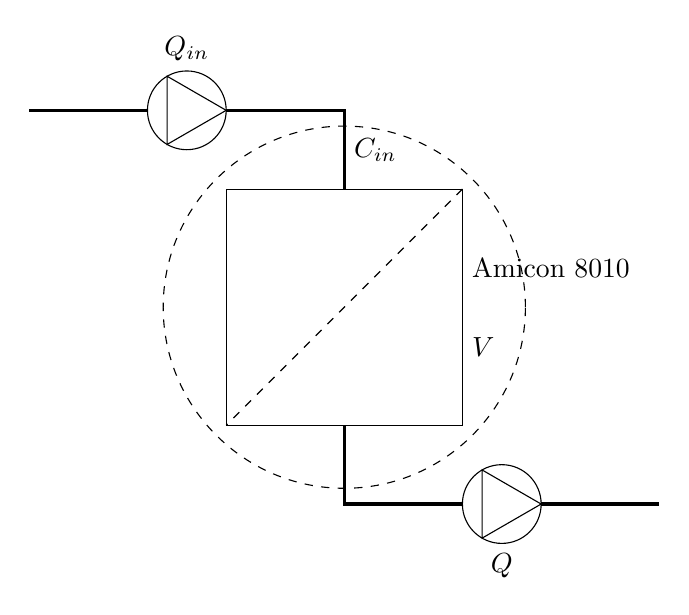
\begin{tikzpicture}

\node[right] at (6, 5) {Amicon 8010};
\node[right] at (6, 4.5) {\concb};
\node[right] at (6, 4) {$V$};
\node[right] at (4.5, 6.5) {$C_{\mr{in}}$};
\node[right] at (4.5, 2.5) {\concp};
 
%\draw[help lines] (0cm, 0cm) grid (10cm, 10cm);

\draw (3, 3) rectangle (6, 6);

\draw[dashed] (6, 6) -- (3, 3);

\draw (2.5, 7) circle (0.5cm);
\node[above] at (2.5, 7.5) {$Q_{\mr{in}}$};
\draw (2.25, 7.433) -- (2.25, 6.567) -- (3, 7) -- cycle;
\draw[very thick] (0.5, 7) -- (2, 7); 
\draw[very thick] (3, 7) -- (4.5, 7) -- (4.5, 6);


\draw (6.5, 2) circle (0.5cm);
\draw (6.25, 2.433) -- (6.25, 1.567) -- (7, 2) --cycle;
\node[below] at (6.5, 1.5) {$Q$};
\draw[very thick] (4.5, 3) -- (4.5, 2) -- (6, 2);
\draw[very thick] (7, 2) -- (8.5, 2);

\draw [thin, dashed] (4.5, 4.5) circle (2.3cm);

\end{tikzpicture}
	\caption[Nomenclatura para balanço de massa na célula Amicon 8010]{Nomenclatura usada para efetuar o balanço de massa durante uma filtração na célula Amicon 8010. Assume-se que não ocorre adsorção na membrana.}
	\label{fig:bal_massa}
\end{figure}

\subsection{Balanço de massa: modo de concentração} % (fold)
\label{sub:modo_con}\index{Amicon 8010!modo de concentração}
Em modo de concentração, $Q_{\mr{in}}=0$ e a equação~\ref{eq:balanco_massa_principal} pode ser reescrita da seguinte forma:
\begin{equation}
	\label{eq:bal_mas_conc_ini}
	-Q\concp=\concb\frac{dV}{dt}+V\frac{d\concb}{dt}
\end{equation}
Para integrar a equação é necessário primeiro determinar a taxa temporal de variação do volume no interior da célula ($dV/dt$). Para isso pode ser feito um balanço de massa à solução. Se for considerado que a densidade da solução se mantém aproximadamente constante durante a filtração, o balanço de massa é dado por:\index{solução!balanço de massa}
\begin{equation}
 	\begin{aligned}
 	dV/dt & = -Q\\
 	    V & = V_0-Qt
 	\end{aligned}
\end{equation}
Introduzindo o anterior resultado na equação~\ref{eq:bal_mas_conc_ini} e integrando a equação entre 0 e $t$ obtém-se:
\begin{equation}
	\label{eq:bal_con_cb}
	\concb=C_{\mr{b0}}\left( 1-\frac{Q}{V_0}t\right)^{\permobs-1}
\end{equation}
em que \concb\ é a concentração do soluto no interior da célula, para um determinado tempo $t$, $C_{\mr{b0}}$ é a concentração inicial do soluto no interior da célula (para $t=0$), $V_0$ é o volume inicial de solução a filtrar no interior da célula e \permobs\ é o coeficiente de permeação observado do soluto, que se assume constante ao longo do tempo e que é definido por:\index{permeação!observada}
\begin{equation}
	\label{eq:permobs_pra}
 	\permobs=\frac{\concp}{\concb}
 \end{equation}
Assim, a equação~\ref{eq:bal_con_cb} permite determinar \permobs\ a partir de valores experimentais de \concb\ e \concp. Sublinhe-se que esta equação é somente válida quando \permobs\ é aproximadamente constante, condição que é normalmente verificada na filtração de solutos neutros e na ausência de colmatação significativa. No caso de solutos com carga elétrica, os valores de \permobs\ não são independentes da concentração no meio, \concb, pelo que a equação~\ref{eq:bal_con_cb} é somente aplicável no caso de pequenas variações de volume, o que é o caso da generalidade das determinações experimentais feitas neste trabalho.
% subsection subsection_name (end)

\subsection{Balanço de massa: modo de diafiltração a volume constante} % (fold)
\label{sub:mod_df}\index{Amicon 8010!modo diafiltração}
No modo de diafiltração a volume constante, o volume de solução no interior da célula permanece constante e a concentração do soluto na corrente de entrada ($C_{\mr{in}}$) é nula. Este modo de operação é muito usado por exemplo para efetuar trocas de tampão de soluções de macromoléculas, sendo uma alternativa ao processo de diálise. Nestas condições, a equação~\ref{eq:balanco_massa_principal} pode ser reescrita da seguinte forma:\index{diálise}
\begin{equation}
	\label{eq:bal_mas_df_ini}
	-Q\concp=V \frac{d\concb}{dt}
\end{equation}
Introduzindo de novo a equação~\ref{eq:permobs_pra}, e considerando \permobs\ constante ao longo do tempo, obtém-se após integração entre 0 e $t$:
\begin{equation}
	\label{bal_mas_df_final}
	\concb=C_{\mr{b0}}\exp \left( -\permobs \frac{Q}{V} t \right)
\end{equation}
Para solutos que apresentem permeabilidades elevadas, a sua concentração no interior da célula decresce exponencialmente ao longo do tempo. Esta equação é particularmente útil para descrever operações de troca de tampão, em que a macromolécula é muito rejeitada enquanto os microsolutos permeiam livremente pela membrana.\index{troca de tampão}
% subsection mod_df (end)

\subsection{Coeficiente de transferência de massa} % (fold)
\label{sub:coef_massa_pra}\index{coeficiente!de transferência de massa}\index{Amicon 8010!coeficiente de transferência de massa}
Outro aspeto muito importante de qualquer processo de filtração é o valor do coeficiente de transferência de massa na camada de polarização de concentração, junto à membrana, o qual foi definido na secção~\ref{sec:filmepol}, através da equação~\ref{eq:kmassa}. De facto, muito do esforço de desenvolvimento e investigação na área das tecnologias de membranas é focalizado na modelação teórica dos processos de transferência de massa ao nível da camada de polarização de concentração, recorrendo a métodos computacionais de dinâmica de fluidos. O desenvolvimento de métodos nessa área vai para além dos objetivos propostos para trabalho de doutoramento, sendo usadas aqui correlações semi-empíricas frequentemente utilizadas na literatura para a estimativa de coeficientes de transferência de massa em casos concretos, as quais são válidas para determinados tipos de equipamento. De acordo com o anteriormente exposto, um coeficiente de transferência de massa elevado é desejável porque permite reduzir os fenómenos de polarização de concentração, tal como referido no capítulo~\ref{chap:teov3}. Uma polarização de concentração excessiva pode originar uma prematura colmatação das membranas, alterando quer a produtividade quer a seletividade destes processos ao longo do tempo. Conduz ainda a um aumento da periodicidade da lavagem e substituição das membranas, facto que gera um elevado impacto económico e ambiental.\index{polarização de concentração}

O coeficiente de transferência de massa, $k$, é fundamentalmente dependente do coeficiente de difusão do soluto, da densidade e viscosidade da solução para além de parâmetros relacionados com o equipamento de filtração, os quais influenciam marcadamente as condições hidrodinâmicas, sendo usualmente determinado por correlações do tipo \cite{mulder}:
\begin{equation}
	\label{eq:k_mulder}
	\mr{Sh}=a\reynolds^b\mr{Sc}^c    	
\end{equation}
onde $\mr{Sh}$, $\reynolds$ e $\mr{Sc}$ são os parâmetros adimensionais número de Sherwood, número de Reynolds e número de Schmidt, respetivamente, e $a$, $b$ e $c$ constantes empíricas. Para a célula de filtração Amicon 8010 pode ser usada a correlação proposta por Opong e Zydney \cite{opong}:
\begin{equation}
	\label{eq:pra_opong}
	\mr{Sh} = 0.23 \reynolds^{0.567} \mr{Sc}^{0.33}
\end{equation}
em que os parâmetros adimensionais são definidos da seguinte forma:
\index{número!de Reynolds}\index{número!de Scmidt}\index{número!de Sherwood}
\begin{equation}
\begin{aligned}
	\mr{Sh}   & = \frac{k\raiocelula}{D} \\
  \reynolds & = \frac{\agitacao\raiocelula^2\densidade}%
		{\viscosidade} \\
	\mr{Sc}   & = \frac{\viscosidade}{\densidade D}
\end{aligned}
\end{equation}
onde \raiocelula\ é o raio da célula de filtração (para a célula Amicon 8010 equivale a 12.5\,mm), $D$ é o coeficiente de difusão, \agitacao\ é a velocidade de agitação em rad/s, \densidade\ é a densidade, e \viscosidade\ a viscosidade dinâmica. Os parâmetros são todos referentes a uma situação não-confinada da solução.\index{raio!da célula}\index{Amicon 8010!raio}

O coeficiente de transferência de massa pode também ser determinado experimentalmente, a partir de valores de \permobs\ obtidos a diferentes fluxos de permeação, se for considerado o modelo do filme (secção~\ref{sec:filmepol}). A equação~\ref{eq:sobsvssm} pode ser usada para determinações diretas. Após alguma manipulação algébrica pode ainda obter-se a seguinte relação, a partir da equação~\ref{eq:sobsvssm}:
\begin{equation}
	\label{eq:pra_sobs2sm_lin}
	\ln \left( \frac{1-\permobs}{\permobs} \right) = 
	\ln \left( \frac{1-\permm}{\permm} \right) - \frac{\fluxo}{k}	
\end{equation}
\index{modelo!do filme}\index{modelo!FJC|see{FJC}}\index{modelo!CSC|see{CSC}}\index{modelo!WLC|see{WLC}}% 
Esta relação prevê uma variação linear entre $\ln[(1-\permobs)/\permobs]$ e o fluxo de filtração, sendo o declive dado por $-k^{-1}$, para o caso de se ter \permm\ constante.
% subsection coef_massa_pra (end)

\subsection{Caracterização de membranas e determinação de coeficientes de permeação} % (fold)
\label{sub:car_mem}\index{caracterização!membranas}
\index{seletividade!membranas}%
Devido às suas características, tais como a facilidade de operação e a reduzida área de membrana necessária, a célula Amicon 8010 revela-se bastante útil para proceder à caracterização de membranas quanto ao seu tamanho de poro. Nesta secção é descrito o procedimento efetuado no presente trabalho para efetuar esta tarefa. Este procedimento foi ainda utilizado para a determinação experimental de valores de coeficiente de permeação observada (\permobs).

Antes de se iniciar uma filtração devem ser efetuados alguns procedimentos de lavagem, quer da célula quer da membrana. Isto pode ser feito operando a célula em modo de pressão constante. Deve ser usada nas lavagens uma água desmineralizada e microfiltrada, sendo que no presente trabalho foi usada água MilliQ (\emph{Millipore}). Para determinar \permobs\ para um determinado soluto, o procedimento usado foi o seguinte:
\index{procedimento!seletividade}
\begin{enumerate}
	\item Colocar a solução a filtrar (mínimo 5\,mL na célula Amicon 8010), da qual se recolhe uma amostra para posterior análise. 
	\item Ajustar a velocidade de agitação pretendida, iniciar a filtração e começar a contagem de tempo.
	\item Recolher 0.5--1\,mL de permeado para um tubo, conforme o volume inicial da solução a filtrar. O tempo de filtração relativo à recolha desta primeira fração será denotado $t_1$.
	\item Sem parar a filtração, continuar a recolha para outro tubo. O tempo de filtração relativo à recolha desta primeira fracção será denotado $t_2$ (contado desde o início da filtração) .
	\item Pesar as duas frações e calcular o volume correspondente.
	\item Analisar as duas frações de permeado, a solução inicial e o concentrado que ficar na célula de filtração, quanto ao conteúdo do soluto em questão e determinar a sua concentração usando o método mais adequado (os vários métodos analíticos são descritos mais à frente).
	\item Calcular o valor de \permobs. 
\end{enumerate}
Usando a equação~\ref{eq:bal_con_cb}, e integrando \concp\ entre o tempo de recolha da primeira fração ($t_1$) e o tempo total de filtração ($t_2$), obtém-se:\index{balanço de massa!seletividade}
\begin{equation}
\label{eq:calcrobs}
C_{\mr{p,med}} = \frac{V_0 C_{\mr{b0}}}{Q(t_1-t_2)}\left[ %
\left(
1 - \frac{Q}{V_0}t_1
\right)^{\permobs} - 
\left(1 - \frac{Q}{V_0}t_2 
\right)^{\permobs}
\right]
\end{equation}\index{permeação!observada}%    
O valor de \permobs\ pode assim ser obtido resolvendo numericamente a equação~\ref{eq:calcrobs}, a partir dos valores de $C_{\mr{p,med}}$ (concentração do soluto na segunda fração) e $C_{\mr{b0}}$ experimentais. Com a concentração do soluto nas duas frações de permeado e os respetivos volumes de permeado pode ainda determinar-se a quantidade total de soluto permeado, a qual pode ser comparada com a quantidade de soluto na amostra inicial e a quantidade de soluto no concentrado final. Isto possibilita verificar se houve ou não adsorção de soluto na membrana, e quantificar a quantidade adsorvida.
% substituindo $C_{\mr{p,med}}$ pelo valor de concentração determinado para a segunda fração de permeado, e substituindo $C_{\mr{b0}}$ pelo valor de concentração do soluto na solução inicial. 

Para caracterizar uma membrana quanto ao seu tamanho de poro é necessário determinar \permobs\ de solutos cujas dimensões moleculares são conhecidas, os quais serão referidos como solutos de referência, seguindo o procedimento descrito em cima, variando entre ensaios a velocidade de agitação e/ou o fluxo de filtração, conforme se revele mais adequado experimentalmente. Os solutos de referência mais usados para caracterizar membranas de UF são dextranos e polietilenoglicóis (PEG's). Para estes dois polímeros podem ser encontradas na literatura correlações para determinar os seus raios hidrodinâmicos (\raiostokes) em função das suas massas moleculares (\massamolecular). Para dextranos \cite{meu1}:\index{dextrano!raio hidrodinâmico}
\index{massa molecular}
\begin{equation}
	\label{eq:rsdextrano_art}
	\raiostokes = 0.0282(\massamolecular)^{0.47752}
\end{equation}
com \raiostokes\ em nm e \massamolecular\ em Da. Para PEG's pode ser usada a seguinte correlação \cite{moraotese}:\index{PEG!raio hidrodinâmico}
\begin{equation}
	\label{eq:rspeg_art}
	\ln \raiostokes = -23.91 + 0.4648 \ln (\massamolecular)
\end{equation}
com \raiostokes\ em m e \massamolecular\ em Da. Estes solutos foram escolhidos porque são neutros e podem ser aproximadamente descritos pelo modelo de esferas rígidas \cite{deen,dechadilok,moraompa}, o que permite a aplicação do modelo do transporte restringido descrito na secção~\ref{sec:restringido}. Desta forma é possível determinar um valor de raio de poro (\raioporo) que minimiza os erros entre os valores de \permobs\ obtidos experimentalmente e os valores obtidos com o modelo, erros estes que podem ser representados por uma função de mínimos quadrados \cite{bowen02}:
\index{raio!do poro}
\begin{equation}
	\label{eq:bowenSy}
	S_y = \sqrt{\frac{\sum_1^n\sum_1^j(S_{\mr{obs,\,exp}}-S_{\mr{obs,\,calc}})^2}{jn-1}}
\end{equation}\index{minimos@mínimos quadrados}%
onde $S_{\mr{obs,\,exp}}$ é a permeação observada determinada experimentalmente, $S_{\mr{obs,\,calc}}$ é a permeação observada calculada pelo modelo, $n$ é o número de solutos usados, cada um com $j$ valores de \permobs\ determinados. Assim, o raio de poro da membrana é determinado como sendo o valor que minimiza $S_y$. 

\section{Principais solutos em estudo} % (fold)
\label{sec:solutos}
Nesta secção é feita a caracterização dos principais solutos em estudo, nomeadamente DNA plasmídico e RNA. É dado ênfase às suas propriedades mais relevantes no âmbito do presente trabalho, ou seja, as propriedades necessárias para a formulação dos modelos apresentados no capítulo~\ref{chap:teov3}. Para além do que é aqui referido, podem ser encontradas na literatura diversas referências que abordam a caracterização pormenorizada destes dois importantes tipos de biomoléculas. De facto, existem revistas científicas totalmente focadas nesta temática, como por exemplo, ``\emph{PLASMID, A Journal of Mobile Genes and Genomes}'' e ``\emph{RNA, A Publication of the RNA Society}''. O texto de Schleef \et\ \cite{schleef} discute as propriedades destas biomoléculas mais relevantes no contexto de um processo de purificação de pDNA.

\subsection{DNA plasmídico} % (fold)
\label{sub:pdna_pra}
\index{DNA plasmídico!propriedades}
Os plasmídeos são moléculas de DNA circulares, de dupla cadeia, que podem ser encontrados maioritariamente em bactérias, onde desempenham várias funções. Em especial, são responsáveis por conferir funções que possibilitam a adaptação destes organismos unicelulares a diferentes meios, conferindo em alguns casos resistência a determinados compostos que atuam como antibióticos. Sendo moléculas de DNA dupla cadeia, o seu tamanho é quase sempre indicado pelo número de pares de bases (nbp) que o constituem. A valores de pH superiores a 4.00 \cite{schleef}, o grupo fosfato em cada base encontra-se ionizado, o que implica que o pDNA apresenta uma elevada quantidade de cargas negativas, mais especificamente 2 cargas negativas por cada par de bases. A sua massa molecular é dependente não só do número de pares de bases mas também da própria constituição em termos do tipo de bases. Neste trabalho opta-se por se utilizar uma aproximação ao valor real da massa molecular do plasmídeo, considerando uma massa molecular média, por par de bases, igual a 660\,Da \cite{prazeresdif}, ou seja:
\index{DNA plasmídico!massamolecular}
\index{massa molecular}
\begin{equation}
\label{eq:mw_pdna_pra}
\massamolecular = 660 (\numpb)
\end{equation}
onde \massamolecular\ é a massa molecular do pDNA em Da. A grande maioria dos plasmídeos apresenta um tamanho que pode ir de 1 kbp a 200 kbp. Devido às suas elevadas dimensões, estas moléculas apresentam valores reduzidos de coeficiente de difusão. No presente o trabalho, os coeficientes de difusão das moléculas de pDNA estudadas foram determinados pela correlação proposta por Prazeres \cite{prazeresdif}:
\index{DNA plasmídico!coeficiente de difusão}
\index{coeficiente!de difusão}
\begin{equation}
\label{eq:prazeres_dif_pra}
\begin{gathered}
	D = A\frac{T}{\eta}(\numpb)^{-2/3} \\
	A = 3.31 \times 10^{-15}\, \mr{N}/\mr{K}
\end{gathered}
\end{equation}
onde $T$ é a temperatura absoluta da solução (K), $\eta$ a viscosidade (Pa$\cdot$s), nbp é o número de pares de bases do plasmídeo e $A$ é uma constante empírica determinada pelo autor.\index{temperatura}
\index{número!pares de bases} 

Sendo moléculas carregadas negativamente, os plasmídeos apresentam variações no seu tamanho consoante a força iónica do meio, facto que é causado pela redução da intensidade das forças eletrostáticas repulsivas, entre os seus grupos carregados, na presença de sais. Este efeito, no caso de moléculas de DNA, pode ser contabilizado pela correlação proposta por Manning \cite{manning}:
\index{força iónica}
\index{comprimento!inverso Debye}
\index{comprimento!persistência}
\index{comprimento!de Bjerrum}
\index{raio!dupla hélice}
\begin{equation}
\label{eq:manning_pra}
\persis=\left(\frac{\pi\persis^{*}}{2}\right)^{2/3}\frac{\raioduplahelice^{4/3}}{\cargaeletrica^{2}\bjerrum}\left[(2\cargaeletrica\densidadecarga-1)\frac{\inversodebye b \numeroeuler^{-\inversodebye b}}{1-\numeroeuler^{-\inversodebye b}}-1-\ln(1-\numeroeuler^{-\inversodebye b})\right]
\end{equation}
onde $a$ é o comprimento de persistência do DNA, contabilizando a presença das suas cargas negativas, $\persis^{*}$ é o comprimento de persistência de um isómero da molécula de DNA para o qual os grupos fosfato não estão ionizados (ver \cite{manning}), \raioduplahelice\ é o raio da dupla hélice do DNA, \cargaeletrica\ é a valência do catião do sal presente em solução, \bjerrum\ é o comprimento de Bjerrum da água pura, \densidadecarga\ é a densidade de carga do DNA e $b$ é o espaço entre cargas no DNA. Os valores que podem ser usados para os vários parâmetros são \cite{latu09,manning}:
\begin{equation}
\label{eq:prop_manning_pra}
\begin{aligned}
  \persis^{*} & = 7.5\,\mr{nm} \\
  \raioduplahelice & = 1\,\mr{nm} \\
  \bjerrum & = 0.71\,\mr{nm} \\
  \densidadecarga & = 4.2 \\
  b & = 0.17\,\mr{nm}
\end{aligned}  	
\end{equation}
\index{DNA plasmídico!raio dupla hélice}
\index{DNA plasmídico!densidade carga}
\index{DNA plasmídico!comprimento de persistência}% 
A variação do comprimento de persistência com a força iónica da solução está implícita no valor do inverso do comprimento de Debye, \inversodebye, que pode ser calculado, em unidades SI, por \cite{manning}:
\begin{equation}
\label{eq:inverso_debye_pra}
\inversodebye = \sqrt{8\pi\avogadro\bjerrum\forcaionica}
\end{equation}\index{número!de Avogadro}%
onde $\avogadro$ é o número de Avogadro e $\forcaionica$ o valor da força iónica da solução. Para determinar o raio de giração das moléculas de pDNA opta-se, no presente trabalho, por as representar como cadeias fechadas segmentadas (capítulo~\ref{chap:teov3}). Seguindo esta abordagem, foi possível obter uma relação entre o raio de giração e o comprimento de persistência e número de pares de bases do plasmídeo, encontrando-se os detalhes inerentes à obtenção da seguinte relação explicitados no capítulo~\ref{chap:art2}:
\index{DNA plasmídico!raio de giração}
\begin{equation}
\label{eq:rg_a_nbp_pra}
\begin{gathered}
\raiogiracao = c_1 a ^ {c_2} \numpb ^ {1-c_2} \\
c_1 = 1.1631 \times 10 ^ {-7};\ \ c_2 = 0.352
\end{gathered}
\end{equation}
com \raiogiracao\ e $a$ em m. O comprimento de persistência pode ser calculado com a equação~\ref{eq:manning_pra}. Na tabela~\ref{tab:prop_pdna_pra} encontram-se os três plasmídeos utilizados no presente trabalho, bem como as suas propriedades mais relevantes, calculadas pelas equações apresentadas.
\begin{table}
	\centering
	\caption[Propriedades mais relevantes dos plasmídeos estudados]{Propriedades mais relevantes, no âmbito do presente trabalho, dos três plasmídeos estudados.}
	\label{tab:prop_pdna_pra}
\begin{threeparttable}
\begin{tabular*}{0.85\textwidth}{l@{\extracolsep{\fill}} d{1} d{7} d{12} d{7} }
 \toprule
Plasmídeo & \mc{1}{l}{\numpb\phantom{nnn}} & \mc{1}{l}{\massamolecular\,[MDa]} &\multicolumn{1}{l}{$D \times 10^{12}$\,[m$^2$/s]}&\multicolumn{1}{l}{$\raiogiracao\times 10^9$\,[m]}\\
\midrule
\pUC     & 2686  & 1,77 & 5,76 & 53,3  \\
\pVAX    & 6050  & 3,99 & 3,35 & 90,2  \\
\pCAMBIA & 12361 & 8,16 & 2,08 & 143,3 \\
\bottomrule
\end{tabular*}
\begin{tablenotes}
\item{}$T=298$\,K, $\eta=8.87\times 10^{-3}$\,Pa$\cdot$s
\item{}$I=150$\,mM (NaCl)
\end{tablenotes}
\end{threeparttable}
\end{table}

\subsection{RNA} % (fold)
\label{sub:rna_pra}\index{RNA}
Os lisados obtidos pelo procedimento usado de lise alcalina, descrito na secção~\ref{sec:lise_alcalina}, contêm como principal contaminante moléculas de RNA, o que torna premente o estudo desta biomolécula. Analisando o lisado por eletroforese em gel de agarose (figura~\ref{fig:ef_pra}), observam-se duas bandas distintas de RNA: uma primeira banda com menor distância de migração, que se refere ao RNA ribossómico da \ecoli\ de maior massa molecular (RNA\,23 e 16S), e uma segunda banda onde se podem encontrar moléculas de RNA de menor massa molecular. A primeira banda diz assim respeito ao chamado RNA de alto peso molecular (HMw\,RNA) de que fazem parte o RNA\,16S e 23S. A segunda banda contém o denominado RNA de baixo peso molecular (LMw\,RNA), sendo o RNA\,5S o seu principal constituinte \cite{meu3}.
\begin{figure}
	\centering
	\begin{tikzpicture}

%\draw[help lines] (0cm, 0cm) grid (12cm, 8cm);


% \draw[help lines] (0cm, 0cm) grid (12cm, 8cm);

\node at (2.5cm, 4cm) {%\includegraphics[width=7cm]{% mudar para 6.3 cm
\includegraphics[width=5cm]{ef_pra.jpg}};

\fill[white] (3.7, 1.1) rectangle (5.1, 6.9);

\draw (3.8, 4.7) -- (4.2, 4.7) node[right] {pDNA\,(sc)};
\draw (3.8, 5.15) -- (4.2, 5.15) node[right] {pDNA\,(oc)}; 
\draw (3.8, 2.9) -- (4.2, 2.9) node[right] {HMw\,RNA};
\draw (3.8, 2.0) -- (4.2, 2.0) node[right] {LMw\,RNA}; 



\end{tikzpicture}

	\caption[Identificação dos tipos de RNA na análise de AGE]{Identificação dos dois principais grupos de RNA (HMw e LMw\,RNA) numa análise de lisados por eletroforese em gel de agarose. Na figura encontra-se várias amostrar de um lisado do plasmídeo \pVAX, obtido por lise alcalina.}
	\label{fig:ef_pra}
\end{figure}

As moléculas de RNA, ao contrário dos plasmídeos, são moléculas de cadeia simples. O seu tamanho pode ser indicado pelo número de nucleótidos (nnt) que o constituem. No entanto, para o caso específico das moléculas de RNA, é mais usual proceder à sua identificação através dos valores dos seus coeficientes de sedimentação (s), em operações de ultracentrifugação, avaliados em unidades Svedberg (S). Assim, pela teoria básica da ultracentrifugação, é possível estimar o raio hidrodinâmico em função da massa molecular e do coeficiente de sedimentação \cite{voet,beckman}:
\index{coeficiente!de sedimentação}
\index{número!nucleótidos}
\index{Svedberg}
\begin{equation}
\label{eq:ultracentri_pra}
\raiostokes=\frac{1}{6\pi\viscosidade}\left[ \frac{\massamolecular}{\avogadro}\frac{(1-\volumeparcial\densidade)}{\sedimentacao}\right]
\end{equation}%
\index{volume!parcial específico}%
\index{RNA!volume parcial específico}%
\index{RNA!coeficiente de sedimentação}%
\index{RNA!massa molecular}%
\index{massa molecular}%
\index{RNA!raio hidrodinâmico}%
onde \raiostokes\ representa o raio hidrodinâmico do RNA, \viscosidade\ a viscosidade da solução, \massamolecular\ a massa molecular do RNA, \volumeparcial\ o volume parcial específico do RNA, \densidade\ a densidade da solução e \sedimentacao\ o coeficiente de sedimentação do RNA. A massa molecular do RNA pode ser aproximadamente calculada considerando que cada nucleótido tem uma massa molecular média de 340\,Da.\footnote{\url{http://www.nordicbiosite.com}} O volume parcial específico pode ser considerado aproximadamente constante para os vários tipos de RNA, sendo o seu valor médio de 0.53\,mL/g \cite{beckman}. O coeficiente de difusão pode assim ser obtido a partir dos valores do raio hidrodinâmico através da equação de Stokes-Einstein:
\index{equação!Stokes-Einstein}
\begin{equation}
\label{eq:stokes_einstein_pra}
D=\frac{\boltzman T}{6\pi\viscosidade\raiostokes}
\end{equation}
onde $D$ representa o coeficiente de difusão, \boltzman\ a constante de Boltzmann, $T$ a temperatura absoluta e \viscosidade\ a viscosidade da solução.

No presente trabalho optou-se por representar as várias moléculas de RNA presentes nos lisados pela abordagem de cadeias de ligação livre (capítulo~\ref{chap:art3}). Segundo esta abordagem, o raio de giração pode ser obtido a partir do raio hidrodinâmico através do modelo de Zimm \cite{teraoka,fukatsu,robertson}:\index{FJC}\index{modelo!Zimm}\index{RNA!raio de giração}
\begin{equation}
\label{eq:rs2rg_pra}
\raiogiracao = 1.505 \raiostokes
\end{equation}
Na tabela~\ref{tab:prop_rna_pra} encontram-se as propriedades mais relevantes, no âmbito do presente trabalho, das três espécies de RNA consideradas. 
\begin{table}
	\centering
	\caption[Propriedades mais relevantes das espécies de RNA estudadas]{Propriedades mais relevantes, no âmbito do presente trabalho, das três espécies de RNA estudadas.}
	\label{tab:prop_rna_pra}
\begin{threeparttable}
\begin{tabular*}{\textwidth}{l@{\extracolsep{\fill}} d{0} d{6} d{4} d{7} d{7} d{12}}
 \toprule
RNA & \mc{1}{l}{nnt\phantom{n}} & \mc{1}{l}{$\sedimentacao\times 10^{13}$\,[s]} & \mc{1}{l}{\massamolecular\,[kDa]} & \multicolumn{1}{l}{$\raiostokes\times 10^9$\,[m]} &\multicolumn{1}{l}{$\raiogiracao\times 10^9$\,[m]} & \multicolumn{1}{l}{$D \times 10^{11}$\,[m$^2$/s]}\\
\midrule
RNA\,5S   &  120 &  5 &  40,80 &  3,39 &  5,10 & 7,29 \\
RNA\,16S  & 1541 & 16 & 523,94 & 13,6  & 20,5  & 1,82 \\
RNA\,23S  & 2904 & 23 & 987,36 & 17,8  & 26,8  & 1,39 \\
\bottomrule
\end{tabular*}
\begin{tablenotes}
\item{}$T=298$\,K
\item{}$\eta=8.87\times 10^{-3}$\,Pa$\cdot$s
\end{tablenotes}
\end{threeparttable}
\end{table}

\section{Método de quantificação HIC} % (fold)
\label{sec:hic_pra}\index{HIC}\index{DNA plasmídico!quantificação|see{HIC}}\index{RNA!quantificação|see{HIC}}
Nesta secção são feitas algumas considerações sobre o principal método quantitativo utilizado no presente trabalho. Este método, da autoria de Diogo \et\ \cite{diogo}, é um método de cromatografia por interação hidrofóbica (HIC) e foi originalmente desenvolvido para quantificar o pDNA presente nas várias amostras ao longo de um processo de purificação. Não há distinção entre as várias isoformas de pDNA, pelo que o valor determinado pelo método corresponde ao valor da concentração total de plasmídeo. Os detalhes específicos da execução experimental do referido método são fornecidos nos capítulos~\ref{chap:art3}~e~\ref{chap:art4}.
\begin{figure}
	\centering
	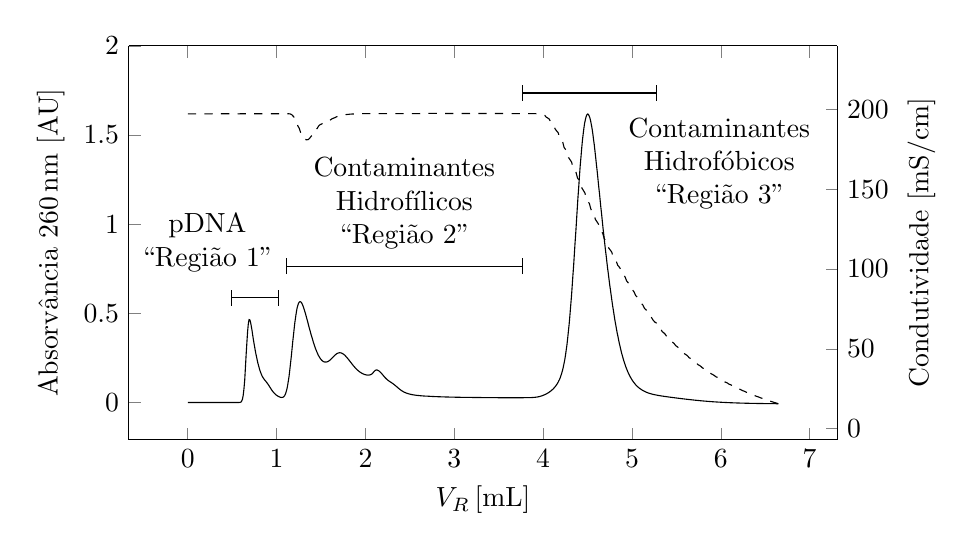
\begin{tikzpicture}

% \draw[help lines] (0cm, 0cm) grid (12cm, 8cm);

\draw (2.3, 2.8) -- (2.9, 2.8) (2.3, 2.7) -- (2.3, 2.9) %
      (2.9, 2.7) -- (2.9, 2.9);

\node[align = center] at (2, 3.5) {pDNA \\ ``Região 1''};

\draw (3, 3.2) -- (6, 3.2) (3, 3.1) -- (3, 3.3) %
      (6, 3.1) -- (6, 3.3);

\node[align = center] at (4.5, 4) {Contaminantes \\%
Hidrofílicos \\ ``Região 2''};

\draw (6, 5.4) -- (7.7, 5.4) (6, 5.3) -- (6, 5.5) %
      (7.7, 5.3) -- (7.7, 5.5);

\node[align = center] at (8.5, 4.5) {Contaminantes \\%
Hidrofóbicos \\ ``Região 3''};


\begin{axis}[%
% xlabel style = {fill = white},
% x tick label style = {fill = white},
width=9cm,
height=5cm,
scale only axis,
axis y line* = left,
% xmin=-5,
% xmax=85,
xlabel={$V_{\mr{R}}$\,[mL]},
% ymin=-500,
ymax = 2,
ylabel={Absorvância 260\,nm [AU]},
at={(1cm, 1cm)},
anchor=south west,
ylabel near ticks
% legend style={at={(1.03,0.5)},legend columns=1,anchor=west,font=\scriptsize,draw=black,fill=white,legend cell align=left}
]
\addplot[
color=black,
solid
]
table[row sep=crcr]{
0.00000	0.00000\\
0.00800	0.00000\\
0.01700	-0.00001\\
0.02500	-0.00001\\
0.03300	-0.00001\\
0.04200	-0.00001\\
0.05000	-0.00001\\
0.05800	-0.00001\\
0.06700	-0.00001\\
0.07500	-0.00001\\
0.08300	-0.00001\\
0.09200	0.00000\\
0.10000	0.00000\\
0.10800	0.00001\\
0.11600	0.00001\\
0.12500	0.00000\\
0.13300	0.00001\\
0.14100	0.00001\\
0.15000	0.00001\\
0.15800	0.00001\\
0.16600	0.00001\\
0.17500	0.00001\\
0.18300	0.00001\\
0.19100	0.00001\\
0.20000	0.00001\\
0.20800	0.00002\\
0.21600	0.00002\\
0.22500	0.00002\\
0.23300	0.00002\\
0.24100	0.00002\\
0.25000	0.00002\\
0.25800	0.00001\\
0.26600	0.00001\\
0.27500	0.00001\\
0.28300	0.00001\\
0.29100	0.00001\\
0.29900	0.00002\\
0.30800	0.00002\\
0.31600	0.00002\\
0.32400	0.00002\\
0.33300	0.00001\\
0.34100	0.00001\\
0.34900	0.00001\\
0.35800	0.00001\\
0.36600	0.00002\\
0.37400	0.00002\\
0.38300	0.00002\\
0.39100	0.00003\\
0.39900	0.00002\\
0.40800	0.00002\\
0.41600	0.00002\\
0.42400	0.00001\\
0.43300	0.00001\\
0.44100	0.00001\\
0.44900	0.00000\\
0.45800	0.00000\\
0.46600	0.00000\\
0.47400	0.00001\\
0.48300	0.00001\\
0.49100	0.00001\\
0.49900	0.00001\\
0.50700	0.00001\\
0.51600	0.00001\\
0.52400	0.00001\\
0.53200	0.00001\\
0.54100	0.00001\\
0.54900	0.00001\\
0.55700	0.00003\\
0.56600	0.00006\\
0.57400	0.00014\\
0.58200	0.00036\\
0.59100	0.00090\\
0.59900	0.00266\\
0.60700	0.00771\\
0.61600	0.01914\\
0.62400	0.04037\\
0.63200	0.07477\\
0.64100	0.12517\\
0.64900	0.19581\\
0.65700	0.26898\\
0.66600	0.34078\\
0.67400	0.40138\\
0.68200	0.44300\\
0.69000	0.46524\\
0.69900	0.46355\\
0.70700	0.44922\\
0.71500	0.42780\\
0.72400	0.40195\\
0.73200	0.37418\\
0.74000	0.34831\\
0.74900	0.32227\\
0.75700	0.29920\\
0.76500	0.27717\\
0.77400	0.25639\\
0.78200	0.23737\\
0.79000	0.21928\\
0.79900	0.20310\\
0.80700	0.18846\\
0.81500	0.17535\\
0.82400	0.16376\\
0.83200	0.15375\\
0.84000	0.14542\\
0.84900	0.13851\\
0.85700	0.13232\\
0.86500	0.12679\\
0.87400	0.12166\\
0.88200	0.11666\\
0.89000	0.11158\\
0.89800	0.10593\\
0.90700	0.10001\\
0.91500	0.09375\\
0.92300	0.08715\\
0.93200	0.08033\\
0.94000	0.07379\\
0.94800	0.06773\\
0.95700	0.06208\\
0.96500	0.05692\\
0.97300	0.05230\\
0.98200	0.04819\\
0.99000	0.04448\\
0.99800	0.04117\\
1.00700	0.03825\\
1.01500	0.03568\\
1.02300	0.03344\\
1.03200	0.03151\\
1.04000	0.02992\\
1.04800	0.02885\\
1.05700	0.02832\\
1.06500	0.02853\\
1.07300	0.02984\\
1.08100	0.03269\\
1.09000	0.03768\\
1.09800	0.04588\\
1.10600	0.05757\\
1.11500	0.07318\\
1.12300	0.09301\\
1.13100	0.11727\\
1.14000	0.14639\\
1.14800	0.18014\\
1.15600	0.21698\\
1.16500	0.25614\\
1.17300	0.29677\\
1.18100	0.33793\\
1.19000	0.37819\\
1.19800	0.41614\\
1.20600	0.45112\\
1.21500	0.48225\\
1.22300	0.50885\\
1.23100	0.53056\\
1.24000	0.54676\\
1.24800	0.55738\\
1.25600	0.56345\\
1.26500	0.56546\\
1.27300	0.56386\\
1.28100	0.55907\\
1.28900	0.55110\\
1.29800	0.54081\\
1.30600	0.52900\\
1.31400	0.51590\\
1.32300	0.50183\\
1.33100	0.48715\\
1.33900	0.47197\\
1.34800	0.45628\\
1.35600	0.44042\\
1.36400	0.42466\\
1.37300	0.40916\\
1.38100	0.39399\\
1.38900	0.37921\\
1.39800	0.36505\\
1.40600	0.35133\\
1.41400	0.33791\\
1.42300	0.32482\\
1.43100	0.31231\\
1.43900	0.30073\\
1.44800	0.29000\\
1.45600	0.28005\\
1.46400	0.27100\\
1.47200	0.26286\\
1.48100	0.25545\\
1.48900	0.24878\\
1.49700	0.24292\\
1.50600	0.23803\\
1.51400	0.23408\\
1.52200	0.23098\\
1.53100	0.22864\\
1.53900	0.22743\\
1.54700	0.22698\\
1.55600	0.22700\\
1.56400	0.22753\\
1.57200	0.22870\\
1.58100	0.23064\\
1.58900	0.23327\\
1.59700	0.23640\\
1.60600	0.24008\\
1.61400	0.24414\\
1.62200	0.24835\\
1.63100	0.25255\\
1.63900	0.25676\\
1.64700	0.26091\\
1.65600	0.26484\\
1.66400	0.26846\\
1.67200	0.27169\\
1.68000	0.27449\\
1.68900	0.27660\\
1.69700	0.27801\\
1.70500	0.27876\\
1.71400	0.27889\\
1.72200	0.27841\\
1.73000	0.27730\\
1.73900	0.27542\\
1.74700	0.27302\\
1.75500	0.27010\\
1.76400	0.26664\\
1.77200	0.26268\\
1.78000	0.25833\\
1.78900	0.25366\\
1.79700	0.24877\\
1.80500	0.24371\\
1.81400	0.23854\\
1.82200	0.23331\\
1.83000	0.22804\\
1.83900	0.22265\\
1.84700	0.21731\\
1.85500	0.21208\\
1.86300	0.20700\\
1.87200	0.20208\\
1.88000	0.19736\\
1.88800	0.19292\\
1.89700	0.18868\\
1.90500	0.18462\\
1.91300	0.18073\\
1.92200	0.17706\\
1.93000	0.17369\\
1.93800	0.17062\\
1.94700	0.16782\\
1.95500	0.16529\\
1.96300	0.16303\\
1.97200	0.16098\\
1.98000	0.15914\\
1.98800	0.15757\\
1.99700	0.15626\\
2.00500	0.15522\\
2.01300	0.15444\\
2.02200	0.15394\\
2.03000	0.15376\\
2.03800	0.15399\\
2.04600	0.15458\\
2.05500	0.15560\\
2.06300	0.15724\\
2.07100	0.15977\\
2.08000	0.16352\\
2.08800	0.16832\\
2.09600	0.17320\\
2.10500	0.17751\\
2.11300	0.18071\\
2.12100	0.18240\\
2.13000	0.18228\\
2.13800	0.18083\\
2.14600	0.17869\\
2.15500	0.17589\\
2.16300	0.17243\\
2.17100	0.16838\\
2.18000	0.16384\\
2.18800	0.15892\\
2.19600	0.15393\\
2.20500	0.14900\\
2.21300	0.14423\\
2.22100	0.13967\\
2.23000	0.13536\\
2.23800	0.13142\\
2.24600	0.12780\\
2.25400	0.12444\\
2.26300	0.12131\\
2.27100	0.11839\\
2.27900	0.11570\\
2.28800	0.11305\\
2.29600	0.11030\\
2.30400	0.10742\\
2.31300	0.10439\\
2.32100	0.10123\\
2.32900	0.09789\\
2.33800	0.09450\\
2.34600	0.09106\\
2.35400	0.08755\\
2.36300	0.08396\\
2.37100	0.08035\\
2.37900	0.07682\\
2.38800	0.07350\\
2.39600	0.07037\\
2.40400	0.06745\\
2.41300	0.06473\\
2.42100	0.06223\\
2.42900	0.05997\\
2.43700	0.05790\\
2.44600	0.05601\\
2.45400	0.05429\\
2.46200	0.05270\\
2.47100	0.05121\\
2.47900	0.04985\\
2.48700	0.04862\\
2.49600	0.04749\\
2.50400	0.04646\\
2.51200	0.04550\\
2.52100	0.04463\\
2.52900	0.04385\\
2.53700	0.04310\\
2.54600	0.04240\\
2.55400	0.04174\\
2.56200	0.04113\\
2.57100	0.04057\\
2.57900	0.04005\\
2.58700	0.03958\\
2.59600	0.03918\\
2.60400	0.03877\\
2.61200	0.03833\\
2.62100	0.03793\\
2.62900	0.03763\\
2.63700	0.03729\\
2.64500	0.03691\\
2.65400	0.03655\\
2.66200	0.03628\\
2.67000	0.03607\\
2.67900	0.03591\\
2.68700	0.03578\\
2.69500	0.03562\\
2.70400	0.03539\\
2.71200	0.03510\\
2.72000	0.03481\\
2.72900	0.03454\\
2.73700	0.03429\\
2.74500	0.03407\\
2.75400	0.03387\\
2.76200	0.03367\\
2.77000	0.03348\\
2.77900	0.03330\\
2.78700	0.03312\\
2.79500	0.03294\\
2.80400	0.03276\\
2.81200	0.03259\\
2.82000	0.03244\\
2.82800	0.03229\\
2.83700	0.03214\\
2.84500	0.03199\\
2.85300	0.03186\\
2.86200	0.03171\\
2.87000	0.03155\\
2.87800	0.03141\\
2.88700	0.03129\\
2.89500	0.03117\\
2.90300	0.03106\\
2.91200	0.03095\\
2.92000	0.03085\\
2.92800	0.03073\\
2.93700	0.03061\\
2.94500	0.03049\\
2.95300	0.03038\\
2.96200	0.03028\\
2.97000	0.03019\\
2.97800	0.03009\\
2.98700	0.03000\\
2.99500	0.02990\\
3.00300	0.02981\\
3.01200	0.02971\\
3.02000	0.02962\\
3.02800	0.02954\\
3.03600	0.02946\\
3.04500	0.02938\\
3.05300	0.02931\\
3.06100	0.02924\\
3.07000	0.02916\\
3.07800	0.02909\\
3.08600	0.02902\\
3.09500	0.02896\\
3.10300	0.02890\\
3.11100	0.02884\\
3.12000	0.02879\\
3.12800	0.02873\\
3.13600	0.02867\\
3.14500	0.02861\\
3.15300	0.02856\\
3.16100	0.02851\\
3.17000	0.02847\\
3.17800	0.02843\\
3.18600	0.02841\\
3.19500	0.02839\\
3.20300	0.02837\\
3.21100	0.02835\\
3.21900	0.02831\\
3.22800	0.02826\\
3.23600	0.02821\\
3.24400	0.02817\\
3.25300	0.02813\\
3.26100	0.02809\\
3.26900	0.02802\\
3.27800	0.02796\\
3.28600	0.02790\\
3.29400	0.02784\\
3.30300	0.02779\\
3.31100	0.02775\\
3.31900	0.02771\\
3.32800	0.02768\\
3.33600	0.02763\\
3.34400	0.02759\\
3.35300	0.02755\\
3.36100	0.02751\\
3.36900	0.02747\\
3.37800	0.02744\\
3.38600	0.02741\\
3.39400	0.02737\\
3.40300	0.02733\\
3.41100	0.02729\\
3.41900	0.02726\\
3.42700	0.02721\\
3.43600	0.02717\\
3.44400	0.02713\\
3.45200	0.02711\\
3.46100	0.02708\\
3.46900	0.02705\\
3.47700	0.02702\\
3.48600	0.02699\\
3.49400	0.02696\\
3.50200	0.02692\\
3.51100	0.02689\\
3.51900	0.02687\\
3.52700	0.02686\\
3.53600	0.02684\\
3.54400	0.02683\\
3.55200	0.02681\\
3.56100	0.02680\\
3.56900	0.02678\\
3.57700	0.02677\\
3.58600	0.02675\\
3.59400	0.02674\\
3.60200	0.02673\\
3.61000	0.02673\\
3.61900	0.02672\\
3.62700	0.02672\\
3.63500	0.02672\\
3.64400	0.02672\\
3.65200	0.02672\\
3.66000	0.02672\\
3.66900	0.02672\\
3.67700	0.02673\\
3.68500	0.02674\\
3.69400	0.02675\\
3.70200	0.02676\\
3.71000	0.02678\\
3.71900	0.02678\\
3.72700	0.02680\\
3.73500	0.02683\\
3.74400	0.02686\\
3.75200	0.02689\\
3.76000	0.02692\\
3.76900	0.02694\\
3.77700	0.02697\\
3.78500	0.02698\\
3.79400	0.02701\\
3.80200	0.02704\\
3.81000	0.02708\\
3.81800	0.02711\\
3.82700	0.02716\\
3.83500	0.02723\\
3.84300	0.02731\\
3.85200	0.02742\\
3.86000	0.02754\\
3.86800	0.02770\\
3.87700	0.02791\\
3.88500	0.02816\\
3.89300	0.02845\\
3.90200	0.02882\\
3.91000	0.02926\\
3.91800	0.02978\\
3.92700	0.03038\\
3.93500	0.03107\\
3.94300	0.03185\\
3.95200	0.03271\\
3.96000	0.03368\\
3.96800	0.03482\\
3.97700	0.03607\\
3.98500	0.03745\\
3.99300	0.03893\\
4.00100	0.04052\\
4.01000	0.04222\\
4.01800	0.04405\\
4.02600	0.04600\\
4.03500	0.04808\\
4.04300	0.05032\\
4.05100	0.05271\\
4.06000	0.05525\\
4.06800	0.05799\\
4.07600	0.06091\\
4.08500	0.06402\\
4.09300	0.06733\\
4.10100	0.07087\\
4.11000	0.07471\\
4.11800	0.07891\\
4.12600	0.08343\\
4.13500	0.08833\\
4.14300	0.09365\\
4.15100	0.09945\\
4.16000	0.10583\\
4.16800	0.11295\\
4.17600	0.12094\\
4.18500	0.12990\\
4.19300	0.14000\\
4.20100	0.15139\\
4.20900	0.16447\\
4.21800	0.17955\\
4.22600	0.19667\\
4.23400	0.21610\\
4.24300	0.23810\\
4.25100	0.26297\\
4.25900	0.29131\\
4.26800	0.32342\\
4.27600	0.35894\\
4.28400	0.39788\\
4.29300	0.44029\\
4.30100	0.48621\\
4.30900	0.53611\\
4.31800	0.58954\\
4.32600	0.64584\\
4.33400	0.70482\\
4.34300	0.76611\\
4.35100	0.82906\\
4.35900	0.89315\\
4.36800	0.95791\\
4.37600	1.02261\\
4.38400	1.08669\\
4.39200	1.14965\\
4.40100	1.21101\\
4.40900	1.26991\\
4.41700	1.32557\\
4.42600	1.37720\\
4.43400	1.42471\\
4.44200	1.46804\\
4.45100	1.50673\\
4.45900	1.53918\\
4.46700	1.56594\\
4.47600	1.58739\\
4.48400	1.60326\\
4.49200	1.61331\\
4.50100	1.61748\\
4.50900	1.61558\\
4.51700	1.60840\\
4.52600	1.59652\\
4.53400	1.58014\\
4.54200	1.55959\\
4.55100	1.53552\\
4.55900	1.50753\\
4.56700	1.47646\\
4.57600	1.44303\\
4.58400	1.40774\\
4.59200	1.37100\\
4.60000	1.33295\\
4.60900	1.29363\\
4.61700	1.25396\\
4.62500	1.21392\\
4.63400	1.17350\\
4.64200	1.13282\\
4.65000	1.09217\\
4.65900	1.05210\\
4.66700	1.01257\\
4.67500	0.97360\\
4.68400	0.93538\\
4.69200	0.89802\\
4.70000	0.86142\\
4.70900	0.82511\\
4.71700	0.78964\\
4.72500	0.75520\\
4.73400	0.72173\\
4.74200	0.68903\\
4.75000	0.65711\\
4.75900	0.62649\\
4.76700	0.59693\\
4.77500	0.56798\\
4.78300	0.53969\\
4.79200	0.51235\\
4.80000	0.48633\\
4.80800	0.46054\\
4.81700	0.43624\\
4.82500	0.41325\\
4.83300	0.39136\\
4.84200	0.37034\\
4.85000	0.34985\\
4.85800	0.33035\\
4.86700	0.31190\\
4.87500	0.29442\\
4.88300	0.27784\\
4.89200	0.26215\\
4.90000	0.24749\\
4.90800	0.23391\\
4.91700	0.22092\\
4.92500	0.20851\\
4.93300	0.19680\\
4.94200	0.18590\\
4.95000	0.17575\\
4.95800	0.16630\\
4.96700	0.15751\\
4.97500	0.14938\\
4.98300	0.14178\\
4.99100	0.13453\\
5.00000	0.12766\\
5.00800	0.12139\\
5.01600	0.11551\\
5.02500	0.10999\\
5.03300	0.10480\\
5.04100	0.10000\\
5.05000	0.09559\\
5.05800	0.09146\\
5.06600	0.08756\\
5.07500	0.08392\\
5.08300	0.08053\\
5.09100	0.07739\\
5.10000	0.07443\\
5.10800	0.07169\\
5.11600	0.06916\\
5.12500	0.06679\\
5.13300	0.06454\\
5.14100	0.06241\\
5.15000	0.06044\\
5.15800	0.05861\\
5.16600	0.05689\\
5.17400	0.05527\\
5.18300	0.05376\\
5.19100	0.05235\\
5.19900	0.05102\\
5.20800	0.04973\\
5.21600	0.04853\\
5.22400	0.04740\\
5.23300	0.04634\\
5.24100	0.04534\\
5.24900	0.04439\\
5.25800	0.04350\\
5.26600	0.04263\\
5.27400	0.04179\\
5.28300	0.04097\\
5.29100	0.04020\\
5.29900	0.03947\\
5.30800	0.03876\\
5.31600	0.03807\\
5.32400	0.03740\\
5.33300	0.03675\\
5.34100	0.03610\\
5.34900	0.03545\\
5.35800	0.03482\\
5.36600	0.03422\\
5.37400	0.03363\\
5.38200	0.03305\\
5.39100	0.03247\\
5.39900	0.03191\\
5.40700	0.03135\\
5.41600	0.03078\\
5.42400	0.03021\\
5.43200	0.02966\\
5.44100	0.02912\\
5.44900	0.02857\\
5.45700	0.02803\\
5.46600	0.02749\\
5.47400	0.02695\\
5.48200	0.02642\\
5.49100	0.02587\\
5.49900	0.02533\\
5.50700	0.02481\\
5.51600	0.02429\\
5.52400	0.02377\\
5.53200	0.02325\\
5.54100	0.02274\\
5.54900	0.02224\\
5.55700	0.02172\\
5.56500	0.02121\\
5.57400	0.02070\\
5.58200	0.02021\\
5.59000	0.01972\\
5.59900	0.01922\\
5.60700	0.01875\\
5.61500	0.01827\\
5.62400	0.01779\\
5.63200	0.01731\\
5.64000	0.01684\\
5.64900	0.01638\\
5.65700	0.01592\\
5.66500	0.01547\\
5.67400	0.01501\\
5.68200	0.01456\\
5.69000	0.01411\\
5.69900	0.01366\\
5.70700	0.01321\\
5.71500	0.01278\\
5.72400	0.01235\\
5.73200	0.01194\\
5.74000	0.01153\\
5.74800	0.01112\\
5.75700	0.01072\\
5.76500	0.01032\\
5.77300	0.00992\\
5.78200	0.00953\\
5.79000	0.00916\\
5.79800	0.00878\\
5.80700	0.00841\\
5.81500	0.00804\\
5.82300	0.00768\\
5.83200	0.00732\\
5.84000	0.00697\\
5.84800	0.00662\\
5.85700	0.00629\\
5.86500	0.00596\\
5.87300	0.00564\\
5.88200	0.00532\\
5.89000	0.00501\\
5.89800	0.00471\\
5.90700	0.00442\\
5.91500	0.00412\\
5.92300	0.00384\\
5.93200	0.00357\\
5.94000	0.00329\\
5.94800	0.00302\\
5.95600	0.00277\\
5.96500	0.00251\\
5.97300	0.00227\\
5.98100	0.00202\\
5.99000	0.00178\\
5.99800	0.00155\\
6.00600	0.00132\\
6.01500	0.00109\\
6.02300	0.00086\\
6.03100	0.00064\\
6.04000	0.00043\\
6.04800	0.00022\\
6.05600	0.00001\\
6.06500	-0.00019\\
6.07300	-0.00038\\
6.08100	-0.00057\\
6.09000	-0.00076\\
6.09800	-0.00094\\
6.10600	-0.00112\\
6.11500	-0.00129\\
6.12300	-0.00147\\
6.13100	-0.00163\\
6.13900	-0.00179\\
6.14800	-0.00195\\
6.15600	-0.00210\\
6.16400	-0.00225\\
6.17300	-0.00240\\
6.18100	-0.00254\\
6.18900	-0.00269\\
6.19800	-0.00283\\
6.20600	-0.00296\\
6.21400	-0.00309\\
6.22300	-0.00322\\
6.23100	-0.00334\\
6.23900	-0.00346\\
6.24800	-0.00358\\
6.25600	-0.00369\\
6.26400	-0.00380\\
6.27300	-0.00391\\
6.28100	-0.00401\\
6.28900	-0.00411\\
6.29800	-0.00420\\
6.30600	-0.00430\\
6.31400	-0.00440\\
6.32300	-0.00450\\
6.33100	-0.00460\\
6.33900	-0.00469\\
6.34700	-0.00478\\
6.35600	-0.00486\\
6.36400	-0.00494\\
6.37200	-0.00502\\
6.38100	-0.00510\\
6.38900	-0.00516\\
6.39700	-0.00524\\
6.40600	-0.00531\\
6.41400	-0.00538\\
6.42200	-0.00545\\
6.43100	-0.00551\\
6.43900	-0.00558\\
6.44700	-0.00563\\
6.45600	-0.00569\\
6.46400	-0.00575\\
6.47200	-0.00582\\
6.48100	-0.00588\\
6.48900	-0.00594\\
6.49700	-0.00600\\
6.50600	-0.00605\\
6.51400	-0.00609\\
6.52200	-0.00614\\
6.53000	-0.00619\\
6.53900	-0.00624\\
6.54700	-0.00629\\
6.55500	-0.00634\\
6.56400	-0.00639\\
6.57200	-0.00643\\
6.58000	-0.00647\\
6.58900	-0.00651\\
6.59700	-0.00656\\
6.60500	-0.00660\\
6.61400	-0.00664\\
6.62200	-0.00668\\
6.63000	-0.00672\\
6.63900	-0.00676\\
6.64700	-0.00678\\
};
\end{axis}

\begin{axis}[%
width=9cm,
height=5cm,
scale only axis,
at={(1cm, 1cm)},
anchor=south west,
% xmin=-5,
% xmax=85,
axis y line* = right,
axis x line = none,
% ymin=-500,
ymax = 240,
ylabel={Condutividade [mS/cm]},
ylabel near ticks
% legend style={at={(1.03,0.5)},legend columns=1,anchor=west,font=\scriptsize,draw=black,fill=white,legend cell align=left}
]
\addplot[
color=black,
dashed
]
table[row sep=crcr]{
0.00000	197.31800\\
0.01700	197.31700\\
0.03300	197.31400\\
0.05000	197.29700\\
0.06700	197.27200\\
0.08300	197.27400\\
0.10000	197.28600\\
0.11600	197.28900\\
0.13300	197.29900\\
0.15000	197.31700\\
0.16600	197.32600\\
0.18300	197.34200\\
0.20000	197.34200\\
0.21600	197.35400\\
0.23300	197.35100\\
0.24900	197.34500\\
0.26600	197.34900\\
0.28300	197.36500\\
0.29900	197.35600\\
0.31600	197.34400\\
0.33300	197.36200\\
0.34900	197.36200\\
0.36600	197.35900\\
0.38200	197.36200\\
0.39900	197.36400\\
0.41600	197.36900\\
0.43200	197.37100\\
0.44900	197.37000\\
0.46600	197.37000\\
0.48200	197.37100\\
0.49900	197.37300\\
0.51600	197.36900\\
0.53200	197.37000\\
0.54900	197.36900\\
0.56500	197.35000\\
0.58200	197.35800\\
0.59900	197.36100\\
0.61500	197.37500\\
0.63200	197.38100\\
0.64900	197.37200\\
0.66500	197.37300\\
0.68200	197.37000\\
0.69800	197.38000\\
0.71500	197.36800\\
0.73200	197.36300\\
0.74800	197.37700\\
0.76500	197.37800\\
0.78200	197.38400\\
0.79800	197.38900\\
0.81500	197.38000\\
0.83200	197.38100\\
0.84800	197.38400\\
0.86500	197.38600\\
0.88100	197.38700\\
0.89800	197.37700\\
0.91500	197.39100\\
0.93100	197.38600\\
0.94800	197.38400\\
0.96500	197.39800\\
0.98100	197.38700\\
0.99800	197.39400\\
1.01400	197.39000\\
1.03100	197.39100\\
1.04800	197.40600\\
1.06400	197.39300\\
1.08100	197.40200\\
1.09800	197.40600\\
1.11400	197.39400\\
1.13100	197.37300\\
1.14700	197.25900\\
1.16400	196.71700\\
1.18100	195.71600\\
1.19700	194.63000\\
1.21400	192.09700\\
1.23100	189.74000\\
1.24700	188.16200\\
1.26400	185.29000\\
1.28100	183.44300\\
1.29700	182.53500\\
1.31400	181.27600\\
1.33000	181.03700\\
1.34700	181.22300\\
1.36400	182.14500\\
1.38000	183.29200\\
1.39700	184.17500\\
1.41400	186.04800\\
1.43000	187.37700\\
1.44700	188.21700\\
1.46300	189.75800\\
1.48000	190.56600\\
1.49700	190.97200\\
1.51300	191.62400\\
1.53000	191.99700\\
1.54700	192.26600\\
1.56300	192.85000\\
1.58000	193.26900\\
1.59600	193.58100\\
1.61300	194.24400\\
1.63000	194.65000\\
1.64600	194.93900\\
1.66300	195.47800\\
1.68000	195.77000\\
1.69600	195.96400\\
1.71300	196.33100\\
1.73000	196.52100\\
1.74600	196.61200\\
1.76300	196.79700\\
1.77900	196.93100\\
1.79600	197.00700\\
1.81300	197.13600\\
1.82900	197.19700\\
1.84600	197.23300\\
1.86300	197.29400\\
1.87900	197.31800\\
1.89600	197.34300\\
1.91200	197.39900\\
1.92900	197.42900\\
1.94600	197.44600\\
1.96200	197.47300\\
1.97900	197.47400\\
1.99600	197.47000\\
2.01200	197.47300\\
2.02900	197.47500\\
2.04500	197.47000\\
2.06200	197.46600\\
2.07900	197.47100\\
2.09500	197.47200\\
2.11200	197.47300\\
2.12900	197.47100\\
2.14500	197.46900\\
2.16200	197.46900\\
2.17900	197.47100\\
2.19500	197.47200\\
2.21200	197.47500\\
2.22800	197.48100\\
2.24500	197.49000\\
2.26200	197.50600\\
2.27800	197.50400\\
2.29500	197.50900\\
2.31200	197.49300\\
2.32800	197.49700\\
2.34500	197.50500\\
2.36100	197.50300\\
2.37800	197.50700\\
2.39500	197.50300\\
2.41100	197.50100\\
2.42800	197.51300\\
2.44500	197.51000\\
2.46100	197.50200\\
2.47800	197.49700\\
2.49500	197.49700\\
2.51100	197.50800\\
2.52800	197.50800\\
2.54400	197.51200\\
2.56100	197.49900\\
2.57800	197.50300\\
2.59400	197.51400\\
2.61100	197.64200\\
2.62800	197.66000\\
2.64400	197.64200\\
2.66100	197.58500\\
2.67700	197.58800\\
2.69400	197.59500\\
2.71100	197.61300\\
2.72700	197.60500\\
2.74400	197.60200\\
2.76100	197.60300\\
2.77700	197.58900\\
2.79400	197.58500\\
2.81000	197.58900\\
2.82700	197.57400\\
2.84400	197.56900\\
2.86000	197.56800\\
2.87700	197.55100\\
2.89400	197.54200\\
2.91000	197.55300\\
2.92700	197.55000\\
2.94400	197.54700\\
2.96000	197.54700\\
2.97700	197.54400\\
2.99300	197.54400\\
3.01000	197.54100\\
3.02700	197.54500\\
3.04300	197.54800\\
3.06000	197.54200\\
3.07700	197.54900\\
3.09300	197.55000\\
3.11000	197.55200\\
3.12600	197.54500\\
3.14300	197.53600\\
3.16000	197.55200\\
3.17600	197.54500\\
3.19300	197.54200\\
3.21000	197.54100\\
3.22600	197.54200\\
3.24300	197.54500\\
3.25900	197.53500\\
3.27600	197.53800\\
3.29300	197.54000\\
3.30900	197.53900\\
3.32600	197.54700\\
3.34300	197.55200\\
3.35900	197.55200\\
3.37600	197.54800\\
3.39300	197.54300\\
3.40900	197.55000\\
3.42600	197.54600\\
3.44200	197.54200\\
3.45900	197.53900\\
3.47600	197.53000\\
3.49200	197.52700\\
3.50900	197.53000\\
3.52600	197.51600\\
3.54200	197.50400\\
3.55900	197.50400\\
3.57500	197.50500\\
3.59200	197.50400\\
3.60900	197.49100\\
3.62500	197.48900\\
3.64200	197.48900\\
3.65900	197.49000\\
3.67500	197.48800\\
3.69200	197.48700\\
3.70800	197.46900\\
3.72500	197.45100\\
3.74200	197.43400\\
3.75800	197.44500\\
3.77500	197.44200\\
3.79200	197.43800\\
3.80800	197.45100\\
3.82500	197.44100\\
3.84200	197.43200\\
3.85800	197.44200\\
3.87500	197.44000\\
3.89100	197.43900\\
3.90800	197.38100\\
3.92500	197.32900\\
3.94100	197.26300\\
3.95800	196.87200\\
3.97500	196.63000\\
3.99100	196.33900\\
4.00800	195.26500\\
4.02400	194.70800\\
4.04100	194.09300\\
4.05800	192.14000\\
4.07400	191.24200\\
4.09100	190.30200\\
4.10800	187.73300\\
4.12400	186.62400\\
4.14100	185.47000\\
4.15800	182.38900\\
4.17400	181.11000\\
4.19100	179.79900\\
4.20700	176.27900\\
4.22400	174.88400\\
4.24100	173.49700\\
4.25700	169.96300\\
4.27400	168.52900\\
4.29100	167.08600\\
4.30700	163.53800\\
4.32400	162.12000\\
4.34000	160.69300\\
4.35700	157.13200\\
4.37400	155.71900\\
4.39000	154.28400\\
4.40700	150.68400\\
4.42400	149.19700\\
4.44000	147.66500\\
4.45700	144.01500\\
4.47300	142.54700\\
4.49000	141.01200\\
4.50700	137.48000\\
4.52300	136.06200\\
4.54000	134.55500\\
4.55700	131.13300\\
4.57300	129.77200\\
4.59000	128.31700\\
4.60700	125.08600\\
4.62300	123.73200\\
4.64000	122.23000\\
4.65600	119.04900\\
4.67300	117.74100\\
4.69000	116.27500\\
4.70600	113.19700\\
4.72300	111.94600\\
4.74000	110.54800\\
4.75600	107.66400\\
4.77300	106.46500\\
4.78900	105.11100\\
4.80600	102.43500\\
4.82300	101.30700\\
4.83900	99.98900\\
4.85600	97.41900\\
4.87300	96.34100\\
4.88900	95.07200\\
4.90600	92.55900\\
4.92200	91.50000\\
4.93900	90.25200\\
4.95600	87.91000\\
4.97200	86.90600\\
4.98900	85.70000\\
5.00600	83.51100\\
5.02200	82.57000\\
5.03900	81.42100\\
5.05600	79.32400\\
5.07200	78.42600\\
5.08900	77.32900\\
5.10500	75.37900\\
5.12200	74.52100\\
5.13900	73.45600\\
5.15500	71.61800\\
5.17200	70.71600\\
5.18900	69.16100\\
5.20500	67.72300\\
5.22200	66.71800\\
5.23800	66.21800\\
5.25500	63.97500\\
5.27200	63.23900\\
5.28800	62.29400\\
5.30500	60.72600\\
5.32200	60.01800\\
5.33800	59.10100\\
5.35500	57.64300\\
5.37200	56.98200\\
5.38800	56.09100\\
5.40500	54.70400\\
5.42100	54.07900\\
5.43800	53.24400\\
5.45500	51.93600\\
5.47100	51.33600\\
5.48800	50.52600\\
5.50500	49.31200\\
5.52100	48.74600\\
5.53800	47.96200\\
5.55400	46.81600\\
5.57100	46.28100\\
5.58800	45.53400\\
5.60400	44.43600\\
5.62100	43.92500\\
5.63800	43.21400\\
5.65400	42.19500\\
5.67100	41.70400\\
5.68700	41.00800\\
5.70400	40.04800\\
5.72100	39.58800\\
5.73700	38.91000\\
5.75400	37.99700\\
5.77100	37.56100\\
5.78700	36.92700\\
5.80400	36.06000\\
5.82100	35.63700\\
5.83700	35.02500\\
5.85400	34.21800\\
5.87000	33.81700\\
5.88700	33.21800\\
5.90400	32.45800\\
5.92000	32.07900\\
5.93700	31.52300\\
5.95400	30.80200\\
5.97000	30.43100\\
5.98700	29.90900\\
6.00300	29.23800\\
6.02000	28.87800\\
6.03700	28.37600\\
6.05300	27.74700\\
6.07000	27.40600\\
6.08700	26.92900\\
6.10300	26.33400\\
6.12000	26.00600\\
6.13600	25.56200\\
6.15300	24.99700\\
6.17000	24.67500\\
6.18600	24.25100\\
6.20300	23.72900\\
6.22000	23.42000\\
6.23600	23.01000\\
6.25300	22.51800\\
6.27000	22.22400\\
6.28600	21.84000\\
6.30300	21.37300\\
6.31900	21.08900\\
6.33600	20.72600\\
6.35300	20.28700\\
6.36900	20.00900\\
6.38600	19.65800\\
6.40300	19.24400\\
6.41900	18.97900\\
6.43600	18.64300\\
6.45200	18.24900\\
6.46900	17.99200\\
6.48600	17.67900\\
6.50200	17.30400\\
6.51900	17.05100\\
6.53600	16.75100\\
6.55200	16.40500\\
6.56900	16.16800\\
6.58500	15.88000\\
6.60200	15.55400\\
};
\end{axis}

\end{tikzpicture}
	\caption[Cromatograma típico do método de quantificação HIC]{Perfil cromatográfico típico de um lisado alcalino, obtido com o método de HIC desenvolvido por Diogo \et\ \cite{diogo}. No cromatograma podem ser identificadas três regiões distintas. Uma primeira região (região 1) que corresponde às moléculas de pDNA, uma segunda região (região 2) onde eluem compostos com maior tempo de retenção mas que não ficam permanentemente ligados à coluna (contaminantes hidrofílicos) e uma terceira região onde eluem os compostos mais hidrofóbicos (contaminantes hidrofóbicos), cuja eluição só é conseguido reduzindo a força iónica do eluente. Na figura está também representado, a tracejado, o perfil da condutividade do eluido}
	\label{fig:hic_pra}
\end{figure}
O princípio de funcionamento do método de HIC assenta nas diferenças de hidrofobicidade entre os vários constituintes do lisado, encontrando-se um cromatograma típico representado na figura~\ref{fig:hic_pra}.\index{lisado}\index{eluente}\index{contaminantes!hidrofílicos}\index{contaminantes!hidrofóbicos}\index{sulfato de amónio!HIC}\index{coluna cromatográfica}\index{cromatograma}\index{cromatografia!interação hidrofóbica|see{HIC}}\index{procedimento!HIC}\index{lisado!HIC}% 
No momento da injeção, o eluente contém uma elevada quantidade de \sulfatoamonio\ (1.5\,M) para que seja possível intensificar as interações dos vários componentes do lisado com a matriz hidrofóbica da coluna. Ao fim de um determinado tempo, o eluente é instantaneamente substituído para um novo eluente sem a presença de \sulfatoamonio\ para assim eluir as espécies retidas na coluna. Podem ser identificadas três regiões distintas no cromatograma apresentado na figura~\ref{fig:hic_pra}. A primeira região (``região 1'') é constituída por um pico com um máximo de absorvância aos 0.7\,mL de volume de retenção, que se atribui exclusivamente às moléculas de pDNA \cite{sousabab,diogo,gomesboro}, que é uma molécula altamente hidrofílica por natureza. Numa segunda região (``região 2''), elui um grupo de compostos que apresentam um maior tempo de retenção mas que não ficam ligados de forma permanente à coluna. Estes contaminantes são por isso denominados contaminantes hidrofílicos. Finalmente, pode ser identificada uma terceira região (``região 3'') que apresenta um pico com um máximo de absorvância em 4.5\,mL de volume de retenção, pico este que é apenas obtido aquando da mudança de eluente. Isto significa que os compostos que eluem nesta região ficam fortemente ligados na coluna e são por isso denominados contaminantes hidrofóbicos\footnote{É importante notar que a convenção de nomenclatura adotada para os contaminantes presentes no lisado serve apenas o propósito de os identificar, não procurando efetuar uma análise profunda do grau de hidrofobicidade dos mesmos.}. Como discutido no apêndice~\ref{app:2}, é proposto no presente trabalho identificar estes contaminantes como sendo, na grande maioria, constituídos pelas moléculas de RNA presentes nos lisados, o que possibilita obter por este método a simultânea quantificação do pDNA e do RNA.  

\section{Lise alcalina} % (fold)
\label{sec:lise_alcalina}\index{lise alcalina}
Nesta secção descreve-se o procedimento utilizado para efetuar o processo de lise alcalina. Para tentar manter a reprodutibilidade entre ensaios usou-se sempre a mesma concentração mássica de células na suspensão a ser lisada. Esta concentração foi escolhida com base num estudo prévio de estabilidade dos lisados, apresentado no apêndice~\ref{app:1}. 

Na realização do presente trabalho efetuou-se o processo de lise alcalina de forma manual\footnote{Naturalmente, de um ponto de vista de aplicação industrial, o processo de lise terá que ser efetuado de forma automática e de preferência em modo contínuo, sendo relevantes os estudos desenvolvidos por Urthaler \et\ \cite{urthaler}, Meacle \et\ \cite{meacle} e Chamsart e Karnjanasorn \cite{staticmixer} sobre esta matéria.}. O procedimento usado é uma modificação do método originalmente proposto por Birnboim e Doly \cite{birnboim}, e consiste nos seguintes três passos:\index{lise alcalina!procedimento}\index{lise alcalina!referências bibliográficas}
\begin{enumerate}
	\item Ressuspender o pellet de \ecoli\ num volume de tampão de ressuspensão apropriado para obter uma suspensão com uma concentração mássica de 120\,g/L (peso húmido). Regra geral, foram ressuspendidas 480\,mg de células em 4\,mL de tampão de ressuspensão.
	\item Adicionar um volume de tampão de lise, agitar de forma suave e incubar a temperatura ambiente durante 5\,min.
	\item Adicionar um volume de tampão de neutralização, agitar de forma suave e incubar em gelo durante 15\,min. 
\end{enumerate}
\renewcommand\descriptionlabel[1]{\hspace{\labelsep}\textbf{#1}}
A constituição dos três tampões enunciados, bem como o modo de preparação e de manutenção dos mesmos, foi a seguinte:\index{lise alcalina!tampões}
\begin{description}
	\item[Tampão de resuspensão] Solução de 50\,mM de Tris e 10\,mM de EDTA. Ajustar pH para 8.00 através da adição de HCl. Conservar a temperatura ambiente. Verificar o pH do tampão antes de utilizar.
	\item[Tampão de lise] Solução de 0.2\,M de NaOH e 1\,\% (w/w) de SDS. Conservar a temperatura ambiente. Antes de utilizar deve-se verificar a existência de uma possível precipitação de SDS, o que pode acontecer se a temperatura ambiente for reduzida. Em caso de ter ocorrido precipitação deve-se incubar o tampão num banho termostatizado a 37\degreecelsius\ até se verificar a completa dissolução de SDS.
	\item[Tampão de neutralização] Solução de 3\,M de acetato de potássio. Ajustar pH para 5.50 através da adição de ácido acético glacial. Conservar a 4\degreecelsius. Verificar o pH antes de utilizar. 
\end{description}\index{tampão!ressuspensão}\index{tampão!lise}\index{tampão!neutralização}\index{RNase}%
É importante notar que o tampão de ressuspensão não contém RNase, que é por vezes usada para degradar o RNA \cite{qiagen}. Esta opção, como referido no capítulo~\ref{chap:intro}, apresenta algumas limitações do ponto de vista de aplicação industrial e é assim desaconselhável. Para além do estudo prévio anteriormente referido, foi ainda realizado um estudo de caracterização dos lisados centrifugados por cromatografia de exclusão molecular (SEC), eletroforese em gel de agarose (AGE), cromatografia de interação hidrofóbica (HIC) e de análise ao conteúdo proteico (BCA). Este estudo é descrito apêndice~\ref{app:2}.
% section hic (end)
% chapter pra (end)